% $Date$
% $Revision$
% $Author$

% !TEX root = SMV_Technical_Reference_Guide.tex

% -------------------  Introduction ------------------------

\section{Introduction}
This \paper\ documents the physics and associated numerical
algorithms used by Smokeview~\cite{Smokeview_Users_Guide} to
visualize smoke and fire.  Smoke color and opacity are visualized
using quantitative physics based methods.  Flame color at present
is visualized using an arbitrary user specified color palette
where color is mapped to gas temperature. Future work involves
mapping color to a blackbody temperature curve enabling a more
quantitative choice of color for this application.

Realistic visualization of fire calculation methods are important
for applications where one wishes to observe qualitative effects
of fire and smoke rather than determine quantitative
characteristics of data such as temperature or velocity.  This
would be the case for a fire fighter using a computer based fire
fighting simulator. Realistic visualization methods, however,
complement but do not replace other more traditional visualization
methods such as 2D contouring or 3D iso-surfacing which are better
suited for quantitatively analyzing data.

Complete methods for visualizing smoke and fire data taking into
account interactions between light and smoke require the solution
of the radiation transport equation (RTE)~\cite{Siegel:2001} also
called the volume rendering equation in visualization
literature.~\cite{levoy:1988} This equation models how light is
affected after interacting with smoke, a participating medium. In
particular, Smokeview uses the RTE to account for extinction
(absorption plus out-scattering) by the smoke and emission from
the fire.

The form of the RTE used by Smokeview to model smoke and fire
appearance is identical to that used by FDS to model radiative
heat transfer. Smokeview uses an extinction coefficient
appropriate for visible light while FDS use one appropriate for
infrared wavelengths of light.  With the proper extinction
coefficient, however, Smokeview can also view smoke at other
wavelengths, simulating a thermal imager, for example. Smokeview
solves the RTE assuming a gray gas environment. This is the
default solution method for FDS. One other important difference is
that Smokeview requires a solution at only one point at a time
(any arbitrary point though), the observer's viewpoint, while FDS
requires a radiation field, a solution at all points within the
solution domain.  Even so, the solution of this
integro-differential equation for visualization requires
significant computation and memory  resources. Approximations are
required in order to display smoke and fire at interactive frame
rates.  The primary approximation is to take advantage of the low
albedo character of smoke allowing one to either simplify or
eliminate scattering terms in the RTE.

Two techniques discussed for visualizing smoke are slice rendered
and volume rendered methods~\cite{levoy:1988,Engel:2006}.    These
methods both solve a form of the RTE equation.  The integrated
quantity in both cases is radiance, the intensity of light seen by
the observer.  They differ in how the integration path is
partitioned.

The first approach, a slice rendering method,  splits the
integration path at grid planes within a 3D mesh. There is one
partially transparent slice for each plane of simulated data.
Planes are drawn through the data along the coordinate planes or
diagonally to these  planes.   The particular plane drawn is
chosen to be the one most perpendicular to the viewer's line of
sight.  The resulting partially transparent slice planes are drawn
individually and combined by the video hardware to form one image.

The separation distance between slice planes becomes smaller as
more planes are used to simulate a case.  As a result, the
computed opacity values are subject to increased round off error
due to finite precision arithmetic.  In fact, if these planes are
sufficiently close, the computed opacities truncate to zero.   In
this situation, volume rendering methods are required.

The second approach, a volume rendering method, also integrates a
simplified form of the radiation transport equation, but over the
entire data mesh.  The integration occurs from the front of the
solution domain (relative to the observer) to the back, rather
than across just one slice plane. By performing the entire
integral at once instead of in pieces, the volume rendered method
does not suffer from the round off errors of the slice rendered
method.  The intermediate computational terms in the volume
rendered method are stored using full precision arithmetic rather
than 8 bits.  A volume rendered method then computes opacity
across multiple grid planes.  As a result, there is only one plane
of data displayed.  The video hardware is again exploited, but
this time to compute a line integral for each pixel in the
observer's view.  Opacities and color for both methods are
computed using transfer functions using soot density and
temperature data obtained from a fire simulation.

This \paper\ is organized as follows.  A model for visualizing
smoke and fire is discussed.  This model, the radiative transport
equation (RTE), is simplified in several ways, one of which gives
the Beer-Lambert law.  Two methods are then discussed for
visualizing smoke  both using a form of the RTE.  The first
method, slice rendering,  uses a series of partially transparent
slices to represent smoke and fire. The second method, volume
rendering, solves the RTE over the entire domain. Finally, several
areas for which the visualization methods may be improved are
given.

% -------------------  Radiation Transport Equation ------------------------

\section{Radiation Transport Equation}
The model used here to visualize smoke is the radiation transport
equation (RTE)~\cite{Siegel:2001}.  This equation uses radiance to
represent smoke appearance.  Radiance has units of Watts per
square meter per unit solid angle~\si{W/(sr.m^2)}.  The solid
angle accounts for the fact that a light source appears brighter
if it emits a given amount of light through a smaller
cross-sectional area.  This has the interesting implication,
ignoring atmospheric effects and as pointed out in
Ref.~\cite{dutre:2002}, that the sun's radiance appears the same
observed from Earth as from Mars.  The diminished heat flux
\si{(W/m^2} on Mars due to the increased distance from the
sun is exactly offset by the reduced solid angle (\si{sr}) that the
sun's disk subtends.  From a visualization perspective, this
implies that image radiance does not depend on distance from the
observer unless  a participating medium is present to absorb or
scatter  light.  The radiation transport equation discussed in
this section models the change in radiance due to these factors.

\renewcommand{\dx}[1]{\,\mbox{d}#1}
\newcommand{\siga}{ \sigma_a(x) }
\newcommand{\sigt}{ \sigma_t(x) }
\newcommand{\sigs}{ \sigma_s(x) }
\newcommand{\sigts}{ \sigma_t(s) }
\newcommand{\Le}{ C_e(x) }
\newcommand{\Lexo}{ C_e(x,\omega) }
\newcommand{\Lxo}{ C(x,\omega) }
\newcommand{\dLdx}{ \frac{\dx{C}}{\dx{x}}(x)}
\newcommand{\intf}[2]{ \exp\left({\int_{#1}^{#2} \sigts \dx{s}}\right) }
\newcommand{\intff}[2]{ {\int_{#1}^{#2} \sigts \dx{s}} }
\newcommand{\intmf}[2]{ \exp\left({-\int_{#1}^{#2} \sigts \dx{s}}\right) }
\newcommand{\intmff}[2]{ {-\int_#1^#2 \sigts \dx{s}} }
\newcommand{\ddx}{ \frac{\mbox{d}}{\dx{x}} }

The radiation transport equation is used to calculate radiance due
to one or more light sources within a region possibly containing a
participating medium such as smoke~\cite{Siegel:2001}. The change
in radiance along a ray with direction $\omega$ at any one instant
and wavelength may be expressed using

\begin{eqnarray}
\label{eq:fullrte}
 \left(\omega\cdot\nabla\right)\Lxo =
-\underbrace{\siga\Lxo}_\mathrm{absorption}-\underbrace{\sigs\Lxo}_\mathrm{out-scattering}
+ \underbrace{\siga\Lexo}_\mathrm{emission} +
\underbrace{\sigs\int_{4\pi}p(x,\omega,\omega')C_i(x,\omega')\dx{\omega'}}_\mathrm{in-scattering}
\end{eqnarray}

\noindent where  $\Lxo$ represents the  radiance at $x$ along a
direction $\omega$. As illustrated in Fig. \ref{figRadiance}, the
right hand side of (\ref{eq:fullrte}) is split into four
components accounting for absorption, in and out scattering and
emission where $\siga$ is the absorption coefficient, $\sigs$ is
the scattering coefficient, $\Lexo$ is the radiance emitted at $x$
along a direction $\omega$ and $p(x,\omega,\omega')$ is the
fraction of light moving along direction $\omega'$ scattered along
direction $\omega$. Absorption and out-scattering cause radiance
to decrease while emission and in-scattering cause radiance to
increase. The radiance terms $C$, $C_e$ and $C_i$ have units of
\si{W/(m^2.sr)}. The coefficients $\sigma_a$ and $\sigma_s$ have
units of \si{1/m} and specify the time and location dependent
change per unit length to the radiance term to which they are
applied.

\begin{figure}[\figoptions]
\begin{center}
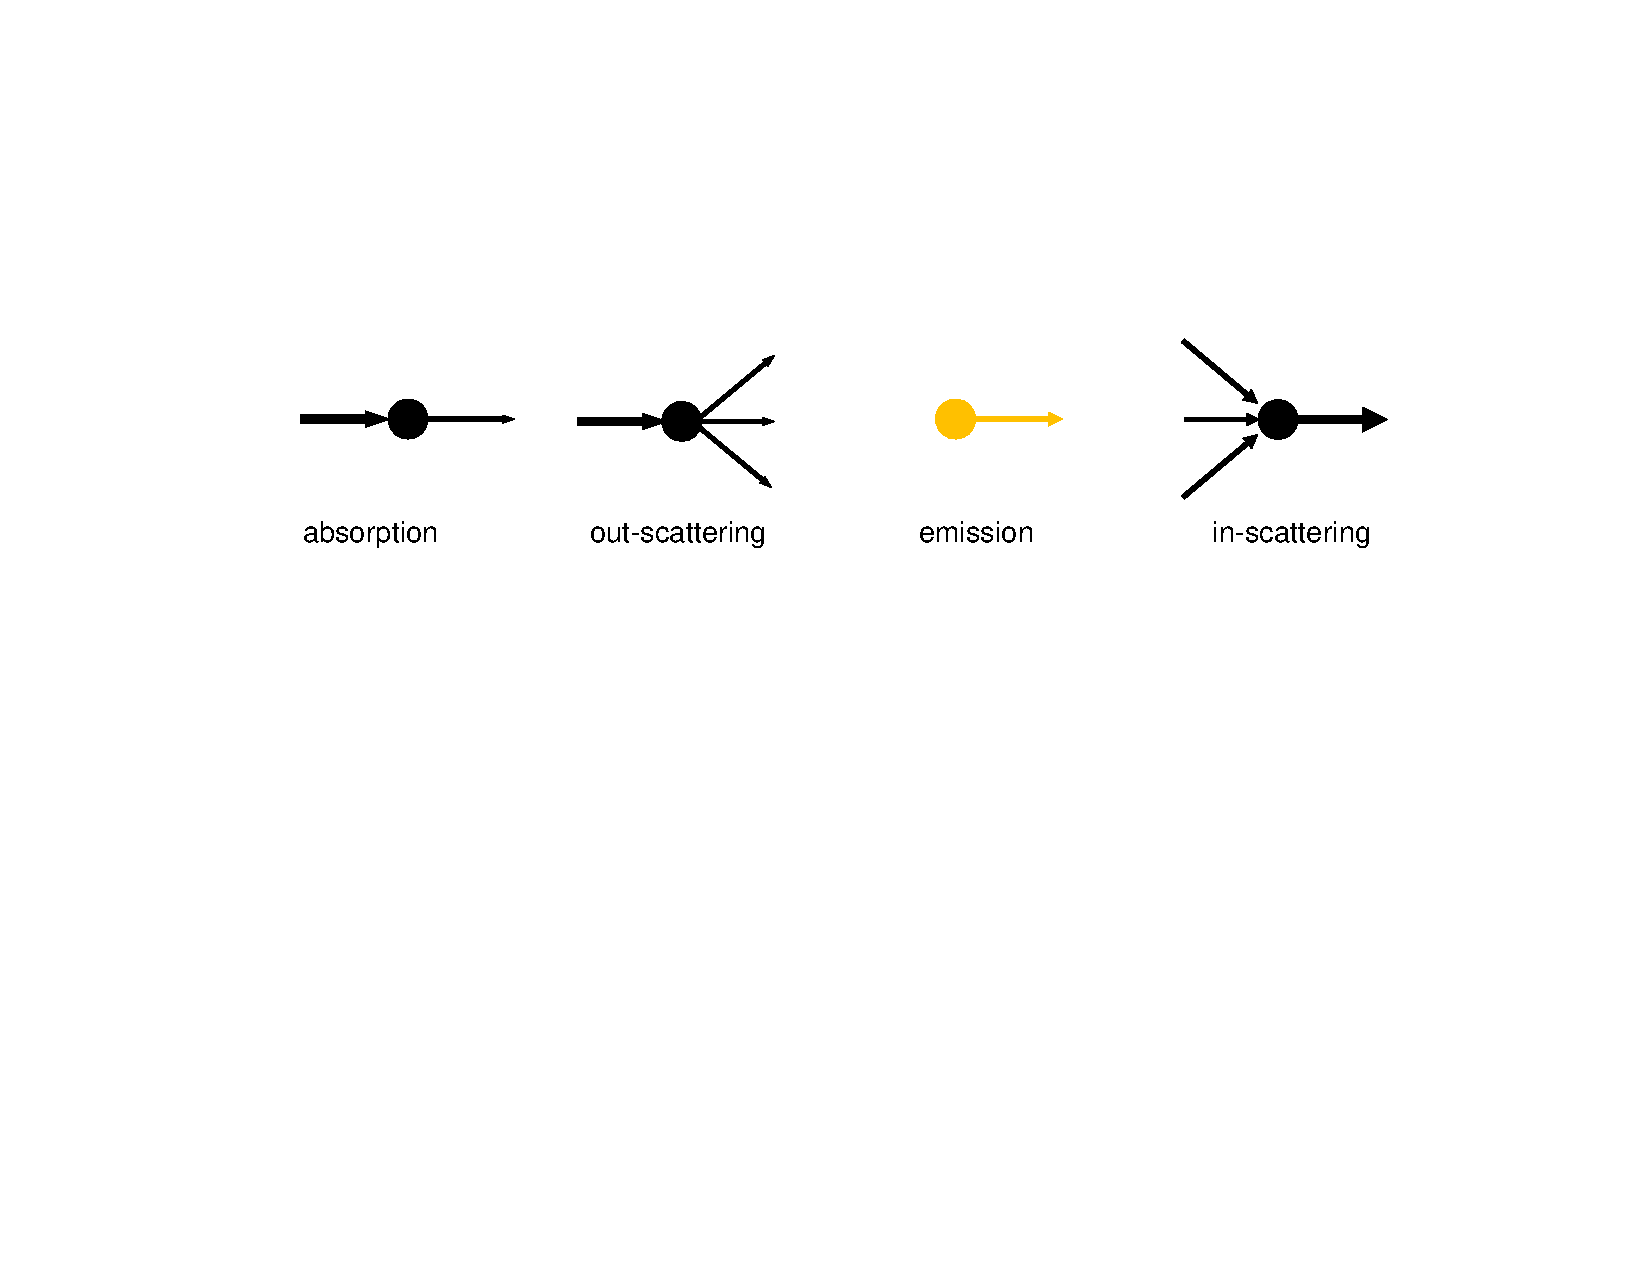
\includegraphics[width=6.0in]{FIGURES/rte_setup}
\end{center}
\caption[Diagram illustrating components of the radiation
transport equation]{Diagram illustrating components of the
radiation transport equation.  Absorption and out-scattering terms
decrease radiance.  Emission and in-scattering terms increase
radiance.} \label{figRadiance}
\end{figure}

% ----  Approximating the Radiation Transport Equation ------------------------

\subsection{Approximating the Radiation Transport Equation}

The RTE may be simplified in several ways depending on which terms
are included or ignored.  This section derives an approximate
solution in which the in-scattering integral term in
(\ref{eq:fullrte}) is neglected and the absorption and
out-scattering coefficients are combined (both are loss terms)
using $\sigt=\siga+\sigs$.  This simplification then only includes
interactions between light and smoke due to absorption,
out-scattering and emission.  Note that the Beer-Lambert law
results if the emission term is also dropped.

Equation (\ref{eq:fullrte}) is then approximated by neglecting the
integral term and using $\sigt=\siga+\sigs$ to obtain

\begin{eqnarray}
\dLdx&=&-\sigt C(x) + \siga C_e(x)\\
 C(x_0)&=&C_0
\end{eqnarray}

This equation may be solved by rearranging terms and applying the
integrating factor $\exp(\int_{x_0}^x \sigts \dx{s})$ obtaining

\begin{eqnarray}
\intf{x_0}{x}\left(\dLdx+\sigt C(x)\right)&=&  \intf{x_0}{x}\siga \Le\\
\ddx\left(\intf{x_0}{x} C(x)\right)&=& \intf{x_0}{x}\siga \Le
\end{eqnarray}

Integrating both sides and substituting the integration limits
results in

\begin{eqnarray}
\left.\intf{x_0}{x} C(x)\right|_{x_0}^{x_N}&=& \int_{x_0}^{x_N}\intf{x_0}{x}\siga \Le \dx{x} \\
\intf{x_0}{x_N} C(x_N)-C_0&=& \int_{x_0}^{x_N}\intf{x_0}{x}\siga \Le \dx{x}
\end{eqnarray}

Solving for $C(x_N)$ after noting that
$\intff{x_0}{x}-\intff{x_0}{x_N}=-\intff{x}{x_N}$ results in

\begin{eqnarray}
C(x_N)&=&\intmf{x_0}{x_N} C_0+ \int_{x_0}^{x_N}\intmf{x}{x_N}\siga
\Le \dx{x}
\end{eqnarray}

\noindent which may be simplified to

\begin{equation}
\label{eq:rtesoln}
 C(x_N)=\tau(x_0,x_N)C_0 + \int_{x_0}^{x_N}\tau(x,x_N)\siga\Le \dx{x}
\end{equation}

\noindent after defining $\tau(a,b)$ as
\begin{equation}
\label{eq:optdepth}
\tau(a,b)=\intmf{a}{b}
\end{equation}
which represents the optical depth between $a$ and $b$.  As noted earlier, if the emission term is neglected and $\sigma_t(x)=\sigma_t$ is constant over a path with length
$L=x_N-x_0$, then (\ref{eq:rtesoln}) simplifies to
\begin{eqnarray}
 \frac{C(x_N)}{C_0}=\exp(-\sigma_tL)
\end{eqnarray}
which is the Beer-Lambert law.

% -------------------  Discretizing the Radiation Transport Equation ------------------------

\subsection{Discretizing the Radiation Transport Equation}
\newcommand{\htau}[1]{\tau_{#1}^{N-1}}
\newcommand{\halpha}[1]{\alpha_{#1}^{N-1}}
\newcommand{\sigai}[1]{\sigma_{a,#1}}
\newcommand{\Lei}[1]{C_{e,#1}}
\newcommand{\Lhatj}[1]{C_{#1}^N}
\newcommand{\Lhatjj}[1]{\hat{C}_{#1}^N}
\newcommand{\Chatjj}[1]{\hat{C}_{#1}^N}
\newcommand{\Leii}[1]{\hat{C}_{e,#1}}

The approximate RTE solution given in (\ref{eq:rtesoln}) is
discretized by converting integral terms into Riemann sums. Figure
\ref{fig:smokediscretesetup}\ illustrates the terms used to
perform these discretizations.  The path is split into $N$ parts
each with length $\Delta x=(x_N-x_0)/N$.  The coordinate system is
set up so that the initial radiance, $C_0$, is located at $x_0$,
most distant from the observer and the final radiance, $C_N$, is
located at $x_N$ closest to the observer.

\begin{figure}[\figoptions]
\begin{center}
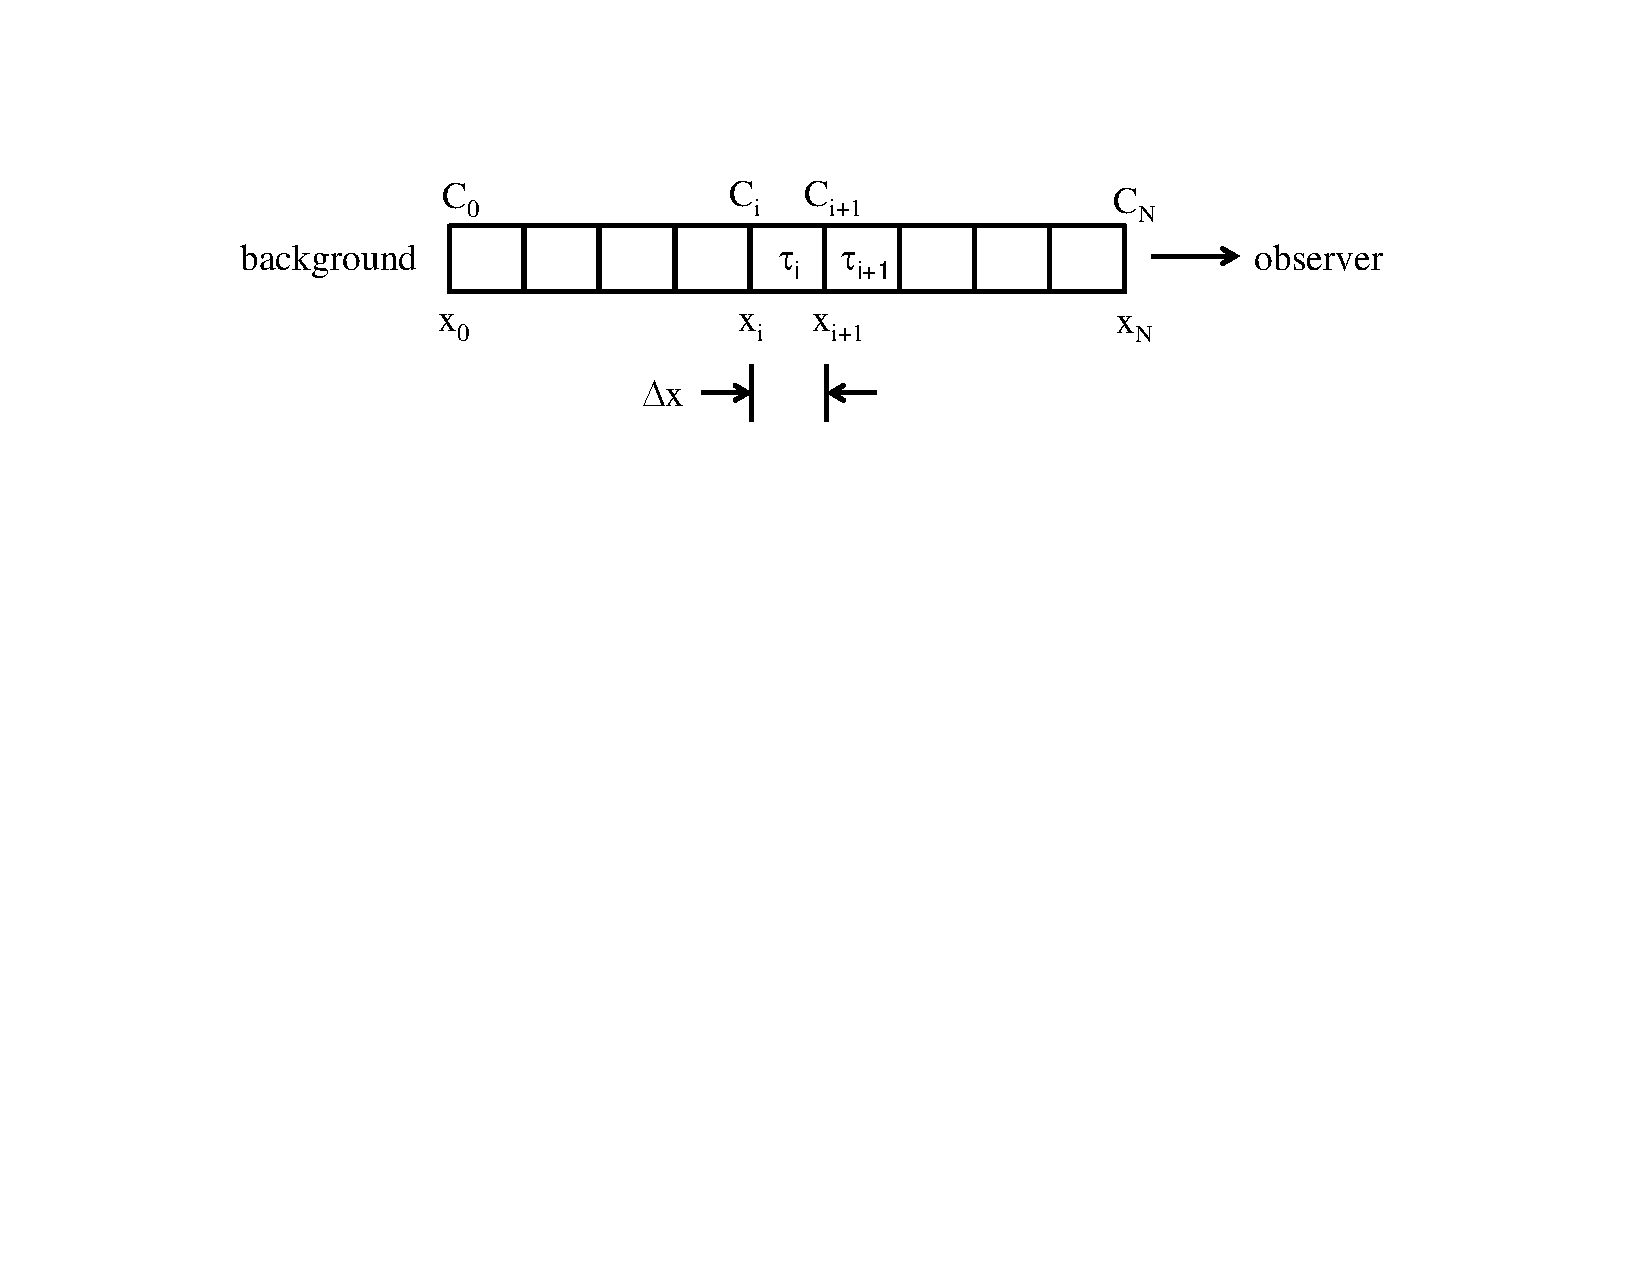
\includegraphics[width=5.0in]{FIGURES/smoke_discrete_setup}
\end{center}
\caption[Setup for discretizing the equations used to model
radiance within a column of 3D smoke data.]{Setup for discretizing
the equations used to model radiance within a column of 3D smoke
data. The transparency across the interval from $x_i$ to $x_{i+1}$
is $\tau_i$. The transparency across the intervals from $x_i$ to
the observer is the product of individual transparencies or
$\tau_i\tau_{i+1}\cdots\tau_{N-1}$} \label{fig:smokediscretesetup}
\end{figure}

The optical depth, $\tau(a,b)$, defined in (\ref{eq:optdepth}) is
discretized using a Riemann sum  after defining sample points
$s_j=x_0+j\Delta s$ for $j=0$ to $N$ with spacing $\Delta
s=(x_N-x_0)/N$ to obtain

\begin{eqnarray}
\htau{i}=\tau(x_i,x_N)&=&\exp\left(-\int_{x_i}^{x_N}\sigma_t(s)\dx{s}\right)\approx\exp\left(-\sum_{j=i}^{N-1}\sigma_t(s_j)\Delta s\right)\\
&=&\prod_{j=i}^{N-1}\exp\left(-\sigma_t(s_j)\Delta s\right)=\prod_{j=i}^{N-1}\tau_j
\end{eqnarray}

\noindent where $\tau_j=\exp\left(-\sigma_t(s_j)\Delta s\right)$
represents the transparency over one discretization interval.
For~$i=N-1$~to~$0$, the optical depth $\htau{i}$ may be computed
recursively using
\begin{eqnarray}
\label{eq:tauhat_recurse}
\htau{i}&=&\htau{i+1}\tau_i
\end{eqnarray}
\noindent where the recursion is initiated with $\htau{N}=1$.
Substituting $1-\halpha{i}=\htau{i}$ and $1-\alpha_i=\tau_i$ into
(\ref{eq:tauhat_recurse}) gives
\begin{eqnarray}
1-\halpha{i}=(1-\halpha{i+1})(1-\alpha_i)=1-\halpha{i+1} - \alpha_i + \halpha{i+1}\alpha_i
\end{eqnarray}
which simplifies to
\begin{eqnarray}
\label{eq:alpha2}
\halpha{i}&=&\halpha{i+1} + (1-\halpha{i+1})\alpha_i
\end{eqnarray}

Similarly, the radiance given by the RTE solution $C(x_N)$ in
(\ref{eq:rtesoln}) may be discretized to obtain

\begin{eqnarray}
C_{N} = \htau{0}\,C_0 +
\sum_{i=0}^{N-1}\htau{i}\,\sigai{i}\,\Lei{i}\,\Delta x
\end{eqnarray}

\noindent where $\sigma_{a,i}=\sigma_a(x_i)$, $\Lei{i}=C_e(x_i)$,
$x_i=x_0+i\Delta x$ and $\Delta x=(x_N-x_0)/N$. This simplifies to

\begin{equation}
\label{eq:discrete_rte2}
C_N = \htau{0}C_0 + \sum_{i=0}^{N-1}\htau{i}\,\Leii{i}
\end{equation}

\noindent where $\Leii{i}=\sigma_{a,i}C_{e,i}\Delta x$.  If
$\Leii{i}$ is interpreted as the emitted color of the fire or
heated gas at location $i$ and $C_0$ is interpreted as the color
of the light source {\em behind}\ the smoke, then
(\ref{eq:discrete_rte2}) restated in words gives color seen by the
observer computed as a weighted average of source and emitted
colors where each weight is the optical depth from the observer to
the corresponding color location.  These emitted colors can be
determined from a blackbody temperature curve or from a colormap
meant to show variations in temperature in terms of color.


The terms in (\ref{eq:discrete_rte2}) are summed from back to
front meaning that the location of the $i=0$ term is farthest from
the observer, while the location of the $i=N-1$ term is closest.
We wish to perform this sum in reverse order, from front to back
so that the sum may be terminated early if additional
contributions would not significantly change the result.

Therefore, to compute $C_N$, let $\Chatjj{j}$ denote the partial
sum using terms $i=j$ through $i=N-1$ in the summation term in
(\ref{eq:discrete_rte2}).  Using this notation
$\hat{C}_N=\htau{0}C_0+\Chatjj{0}$ . Then

\begin{eqnarray}
\label{eq:recurse1}
\Chatjj{j} &= &\sum_{i=j}^{N-1}\htau{i}\,\Leii{i}\\
\label{eq:recurse2}
\Chatjj{j+1}     &= &\sum_{i=j+1}^{N-1}  \htau{i}\,\Leii{i}
\end{eqnarray}

Subtracting (\ref{eq:recurse2}) from (\ref{eq:recurse1}) and solving
for $\Chatjj{j}$ results in
\begin{eqnarray}
\label{eq:color}
\Chatjj{j}&=&\Chatjj{j+1}+\htau{j}\,\Leii{j}
\end{eqnarray}
The strategy then for volume rendering an image is for each pixel
in the 2D projected image to
\begin{enumerate}
\item convert the background radiance $C_0$ to a color,

\item convert the emitted radiances along the integration path to
colors and

\item form a weighted average of these colors using either
equation (\ref{eq:discrete_rte2}) or (\ref{eq:color}) where the
weights are optical depths obtained using (\ref{eq:alpha2}) .

\end{enumerate}
The conversion from radiance to color may be based on a blackbody
temperature curve if realistic flame colors are the goal or
arbitrary if only a qualitative view of the fire is the goal.
Equations (\ref{eq:alpha2}) and ({\ref{eq:color}) are equivalent
to the recursions presented in Ref.~\cite[Chapter 39]{gpugems} for
performing volume rendering.

% -------------------  Splitting the Radiation Transport Equation ------------------------

\subsection{Splitting the Radiation Transport Equation}
This section discusses splitting the Radiation Transport
Equation (RTE), so that it may be solved separately on multiple
meshes or multiple slice planes.  The final solution is then
obtained by  appropriately combining solutions obtained on each
mesh or slice plane.

It is more practical to draw smoke one mesh at a time when
visualizing multiple mesh cases since required data may not be
easily accessible from all meshes, especially if the
GPU\footnote{graphics processing unit of the video card}\ is used
for drawing.  The RTE solution or equivalently the computed
radiance and smoke opacity require  properties for the entire line
of sight which may encompass more than one data mesh.  This
section discusses how  radiance and opacity may be computed by
combining solutions from each individual mesh along the line of
sight.  For example, as illustrated in Fig. \ref{figsmokesetup3},
consider an interval $[x_0,x_N]$ that is split at $D$ into two
sub-intervals $[x_0,D]$ and $[D,x_N]$.  The goal then is to
compute a radiance and opacity for $[x_0,x_N]$ using radiances and
opacities computed on  the two sub-intervals.

\begin{figure}[\figoptions]
\begin{center}
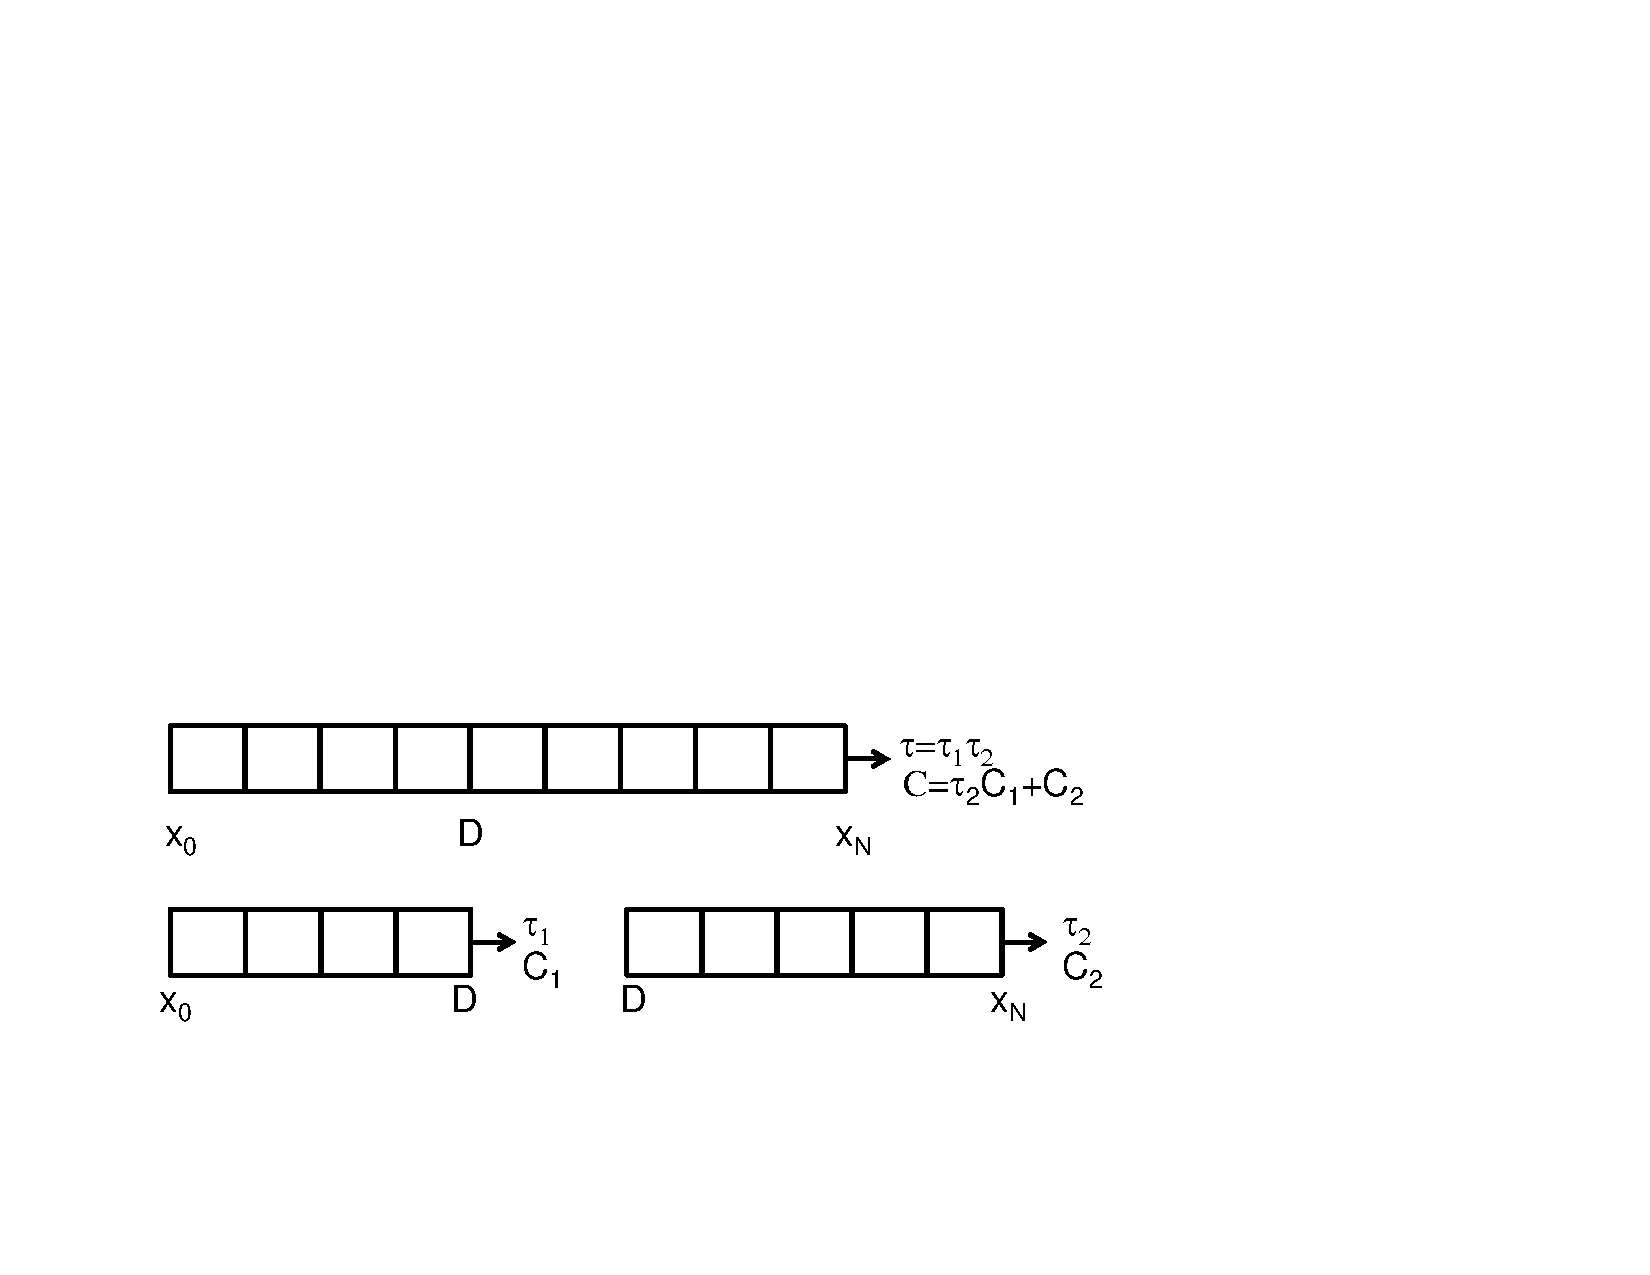
\includegraphics[width=4.0in]{FIGURES/smoke_setup3}
\end{center}
\caption {Solutions to the RTE on two sub-intervals are combined
to form a solution to the RTE for the merger of these intervals.}
\label{figsmokesetup3}
\end{figure}

Let $C$ be a radiance computed on $[x_0,x_N]$ and $C_1$ and $C_2$
be radiances computed on two sub-intervals of $[x_0,x_N]$.
Likewise, let $\tau$ be an optical depth computed on $[x_0,x_N]$
and $\tau_1$ and $\tau_2$ be optical depths computed on two
sub-intervals of $[x_0,x_N]$. From (\ref{eq:rtesoln}) and
(\ref{eq:optdepth}), the radiance $C$ and optical depth $\tau$ are
given by

\begin{eqnarray}
C&=&\int_{x_0}^{x_N}\tau(x,x_N)\sigma_a(x)C_e(x)\dx{x}\\
\tau&=&\tau(x_0,x_N)
\end{eqnarray}

Likewise, the radiances $C_1$ and $C_2$ and optical depths
$\tau_1$ and $\tau_2$ for the intervals $[x_0,D]$ and $[D,x_N]$
are given by

\begin{eqnarray}
C_1&=&\int_{x_0}^{D}\tau(x,D)\sigma_a(x)C_e(x)\dx{x}\\
C_2&=&\int_{D}^{x_N}\tau(x,x_N)\sigma_a(x)C_e(x)\dx{x}\\
\tau_1&=&\tau(x_0,D)\\
\tau_2&=&\tau(D,x_N)
\end{eqnarray}

The optical depth $\tau$ can be split into two parts giving
\begin{eqnarray}
\tau&=&\tau(x_0,x_N)=\tau(x_0,D)\tau(D,x_N)=\tau_1\tau_2
\end{eqnarray}
since from (\ref{eq:optdepth}) it can be shown that for any $x$, $\tau(a,b)=\tau(a,x)\tau(x,b)$.
The radiance $C$ can also be split into two parts giving
\begin{eqnarray}
C&=&\int_{x_0}^{x_N}\tau(x,x_N)\sigma_a(x)C_e(x)\dx{x}\\
&=&\int_{x_0}^{D}\tau(x,x_N)\sigma_a(x)C_e(x)dx+\int_{D}^{x_N}\tau(x,x_N)\sigma_a(x)C_e(x)\dx{x}\\
&=&\tau(D,x_N)\int_{x_0}^{D}\tau(x,D)\sigma_a(x)C_e(x)dx+\int_{D}^{x_N}\tau(x,x_N)\sigma_a(x)C_e(x)\dx{x}\\
&=&\tau_2C_1+C_2
\end{eqnarray}

Summarizing, full-interval values $C$ and $\alpha$ may be written
in terms of sub-interval values $C_1$, $C_2$, $\alpha_1$ and
$\alpha_2$ using

\begin{eqnarray}
\label{eq:alpha_summary}
\tau&=&\tau_1\tau_2\\
\label{eq:C_summary}
C&=&\tau_2C_1+C_2
\end{eqnarray}

Equations (\ref{eq:alpha_summary}) and (\ref{eq:C_summary}) may
then be used to draw smoke and fire one mesh at a time.  These two
equations are also the basis for combining RTE solutions obtained
on multiple slice planes, which is discussed next.

% -------------------  A Solution using Slices ------------------------

\section{Slice Rendering}
A slice rendering algorithm for visualizing smoke consists of
splitting the RTE across individual slice planes within a single
mesh.  The 3D computational domain is partitioned into a series of
2D slices.  The RTE is then solved on each slice.  Each slice
solution only accounts for conditions between adjacent slices.
The individual partially transparent slice solutions are then
combined using video hardware to form the final image.   Problems
can occur with numerical round off error if two slices are too
close together which require solution methods  involving data
volumes rather than data slices. These methods are discussed in
the next section.

There are many ways to slice a 3D data set.  The slice orientation
is chosen to be the one most perpendicular to the viewer's line of
sight, for which possible choices are slice planes parallel to the
three cartesian coordinate planes (XY, XZ, YZ) or planes diagonal
to the data.  The opacity at each grid node is computed using the
distance $\Delta x$ between adjacent YZ planes and soot density
data computed by the fire model.  If slice orientations other than
YZ are displayed, then opacities are adjusted if the distance
between planes is different than $\Delta x$.  Opacity data is
computed and compressed using run length encoding as a
preprocessing step and decompressed one frame at a time as data is
displayed.

% -------------------  Computing Color ------------------------

\subsection{Computing Color}

Smokeview visualizes smoke and fire by drawing a series of triangles in equally spaced parallel planes.  
Color for these triangles are assigned using temperature or hrrpuv (heat release per unit volume) values.
Transparency is assigned using soot density, the greater the soot density, the more opaque the triangle.

An example color map is illustrated in Fig.
\ref{fig:colormaps}.  This maps is split into two parts.  The left half is used
to color non-burning regions, the right half is used to color burning regions.
An hrrpuv cutoff value denoted ${\rm hrrpuv}_{\rm cutoff}$ is used to
determine which half of the color map is used to color a given region.
If an hrrpuv value is below the cutoff
then smoke is drawn using the left have of the color map, otherwise if an hrrpuv value is above the cutoff
then fire colors are drawn using the right half of the color map.  The color map is defined as a table
of 256 red, green, blue color triplets.  A formula giving a color index for a given hrrpuv value is given by

\newcommand{\hrr}{{\rm hrr}}
\newcommand{\hrrcutoff}{{\rm hrr}_{\rm cutoff}}
\newcommand{\hrrmax}{{\rm hrr}_{\rm max}}

\begin{eqnarray}
\mbox{color index}=\left\{
\begin{array}{ll}
  127\frac{\hrr}{\hrrcutoff} & 0 \le \hrr \le \hrrcutoff \\
  127 + 128\frac{\hrr-\hrrcutoff}{\hrrmax-\hrrcutoff} & \hrrcutoff \le \hrr \le \hrrmax
\end{array}
\right.
\end{eqnarray}

\begin{figure}[\figoptions]
\begin{center}

\includegraphics[width=5.0in]{FIGURES/colorbar_fire2}
\end{center}
\caption[Example colormap used for converting temperature or hrrpuv values to color.]
{Example colormap used for converting temperature or hrrpuv values to color.}
\label{fig:colormaps}
\end{figure}

% -------------------  Computing Opacity ------------------------

\subsection{Computing Opacity}
Computing opacity at slice plane nodes is illustrated in Fig.
\ref{figsmokesetup}. A ray travels from the background to the
observer through intervening smoke. Light is absorbed or scattered
by the smoke as the ray passes each slice plane. Emission effects
are accounted for by coloring the smoke.  Scattering effects
presently are only accounted for in the value of the total mass
extinction coefficient.  Light losses are assumed to be from both
absorption and scattering. The obscuration is computed along each
ray one grid plane at a time, using the Beer-Lambert law as
follows.  The $\alpha=1-\tau$ values are pre-computed by FDS using
the Beer-Lambert law~\cite{Siegel:2001}

\begin{equation}
\label{eq:alpha}
\alpha=1-\exp(-\sigma_t\Delta x)
\end{equation}

\noindent for a particular view direction (down the $x$~axis)
where $\Delta x$ is this distance between two grid planes and as
before $\sigma_t=\sigma_a+\sigma_s$ is the total mass extinction
coefficient.  The Beer-Lambert law is an empirical relationship
relating light absorption to the material properties of the medium
the light is travelling through, in this case soot or smoke.

\begin{figure}[\figoptions]
\begin{center}
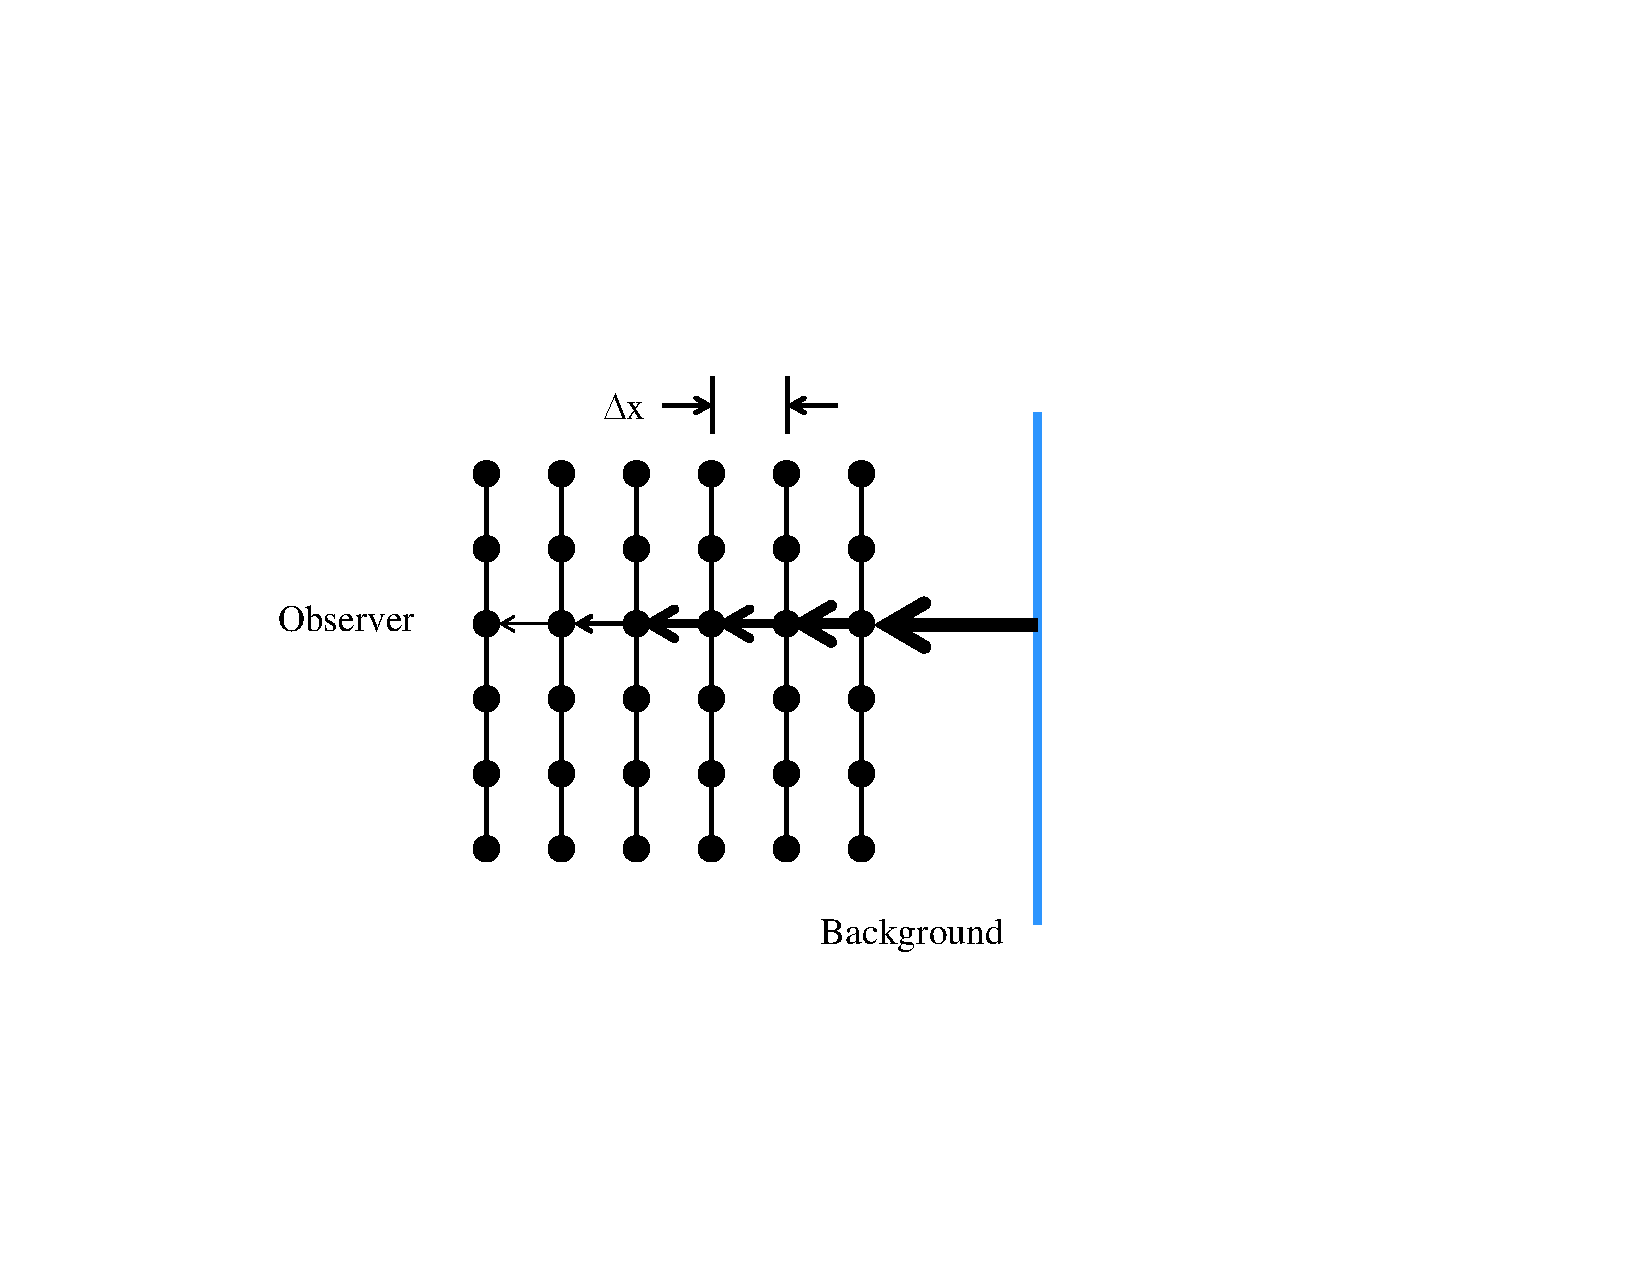
\includegraphics[width=4.0in]{FIGURES/smoke_setup}
\end{center}
\caption[Light emitted from the background is obscured by intervening smoke.]
{Light emitted from the background is obscured by intervening smoke.
}
\label{figsmokesetup}
\end{figure}

The $\alpha$ parameter in (\ref{eq:alpha}) is used by
OpenGL~\cite{OpenGLRed} to blend smoke planes with the current
background.  The $\alpha$ parameter used here also represents an
opacity, 0.0, for completely transparent, and 1.0 for completely
opaque.

% -------------------  Adjusting Opacity ------------------------

\subsection{Adjusting Opacity}

The absorption parameter, $\alpha$, needs to be adjusted for view
directions not aligned with the axis orthogonal to the viewing
planes (see Fig. \ref{figray}).  The absorption coefficient also
needs to be adjusted when the distance between adjacent smoke
planes changes, or viewing planes are skipped.

\begin{figure}[\figoptions]
\centerline{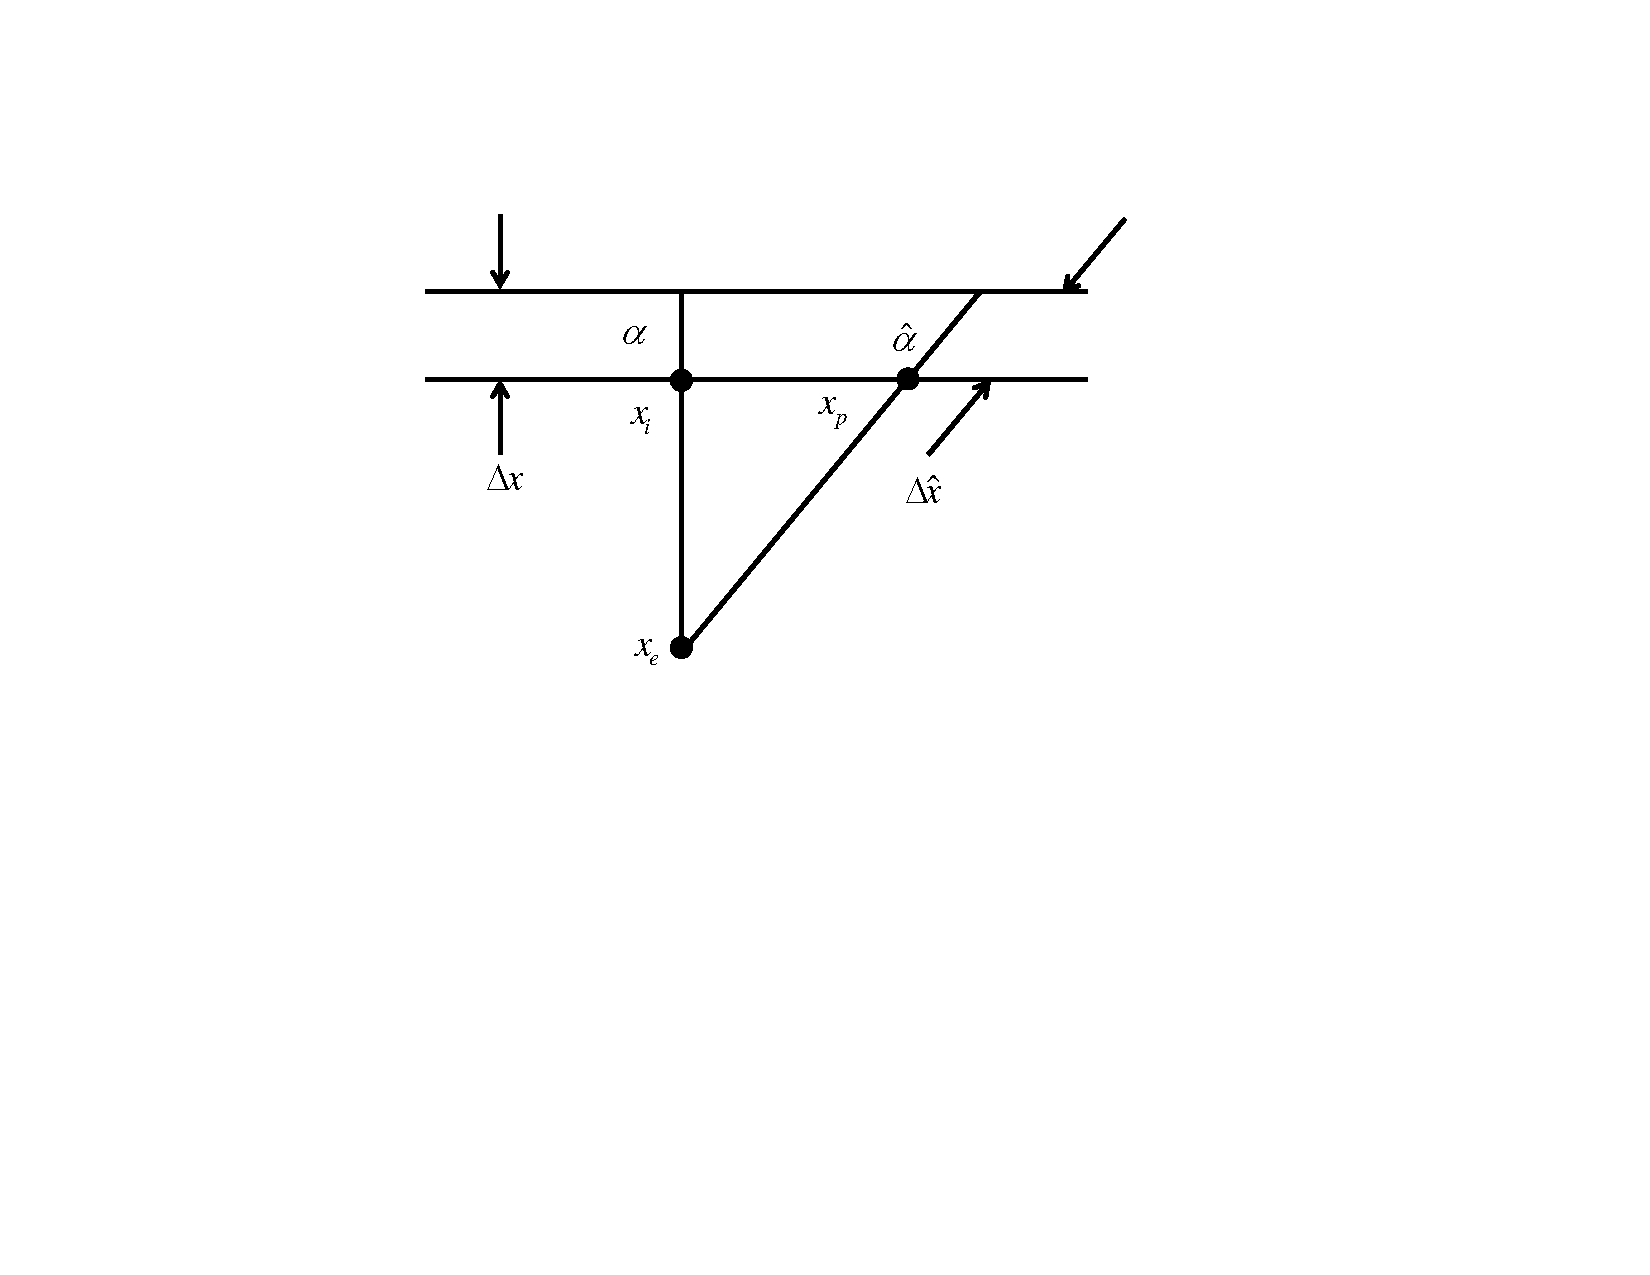
\includegraphics[width=3.5in]{FIGURES/forney_figure4}}
\caption [Diagram illustrating the adjustment required to the
opaqueness parameter, $\alpha$, for non-axis aligned views.] {
Diagram illustrating the adjustment required to the opaqueness
parameter, $\alpha$, for non axis aligned views. The adjusted
opacity $\hat{\alpha}$ along the $\Delta\hat{x}$ segment is
related to $\alpha$ value along the $\Delta x$ segment using
$(1-\hat{\alpha})=(1-\alpha)^{\Delta \hat{x}/\Delta x}$}
\label{figray}
\end{figure}

Ten million exponential operations per second are required to
display smoke with corrected $\alpha$'s at 10 frames per second if
the simulation has grid dimensions of $100\times 100\times 100$.
Recent advances in CPU and video hardware makes these types of
visualizations possible. These corrections may also be performed
in the video card (GPU), resulting in increased display rates
because the GPU performs the corrections simultaneously at all or
many of the grid nodes rather than one at a time as the CPU would.

The $\alpha$ obscurations are pre-computed using the distance
$\Delta x$ between adjacent planes along the $x$~axis. The
adjusted $\hat{\alpha}$ expressed in terms of $\Delta\hat{x}$ is
given by

\begin{equation}
\label{eq:adjusted}
\hat{\alpha}=1-\exp(-\sigma_t\Delta \hat{x})\\
\end{equation}

where $\Delta\hat{x}$ is the distance between planes along the
line of site.  Equations (\ref{eq:alpha}) and (\ref{eq:adjusted})
may be used to solve for $\hat{\alpha}$ in terms of $\alpha$ to
obtain

\begin{equation}
\label{eq:alphahat}
\hat{\alpha}=1-(1-\alpha)^{\Delta\hat{x}/\Delta x}
\end{equation}

after noting that

\begin{eqnarray}
1-\hat{\alpha}=\exp(-\sigma_t\Delta\hat{x})=\exp(-\sigma_t\Delta
x)^{\Delta\hat{x}/\Delta x}=(1-\alpha)^{\Delta\hat{x}/\Delta x}
\end{eqnarray}

The computation of (\ref{eq:alphahat}) is expensive because the
exponential is computed at each grid node for every time step.  In
addition, numerical cancellation may occur for small $\alpha$
leading to loss of significant digits. Both problems may be solved
by expanding (\ref{eq:alphahat}) in a Taylor series and keeping
only the first few terms:

\begin{eqnarray}
\hat{\alpha}\approx \alpha r -
\frac{\alpha^2}{2}r(r-1)+\frac{\alpha^3}{6}r(r-1)(r-2)
\end{eqnarray}

where $r=\sec(\theta)=\Delta \hat{x}/\Delta
x=||x_p-x_e||/n\cdot(x_p-x_e)$, $n$ is the unit vector normal to
the current plane being drawn, $\theta$ is the angle between the
view direction and $n$, $x_e$ is the observers position and $x_p$
is the vertex being drawn (along the view direction).  These terms
are illustrated in Fig. \ref{figray}.

When planes are skipped, (\ref{eq:alphahat}) may be simplified.
In particular, when every 2nd plane is skipped,
$\Delta\hat{x}/\Delta x=2$, so that (\ref{eq:alphahat}) simplifies
to

\begin{eqnarray}
\hat{\alpha}=1-(1-\alpha)^2=2\alpha-\alpha^2
\end{eqnarray}

The video hardware uses $\alpha$ values contained in the smoke
planes to obscure the background much like a camera uses a neutral
density filter to darken a scene.  Extending the analogy,
Smokeview uses one spatial/time varying {\em numerical}\ neutral
density filter for each plane of smoke data.  On a node by node
basis then, each smoke plane obscures the current image stored in
the OpenGL back buffer by the amount $(1-\alpha)$ to form a new
back buffer image.  Figure \ref{figplume} illustrates this process
showing several snapshots of a fire plume. The final image in the
lower right is the most realistic. A simplistic description of one
step of this process is given by

\begin{eqnarray}
\mbox{new buffer image} = (1-\alpha)\times \mbox{old buffer image}
\end{eqnarray}

\begin{figure}[\figoptions]
\begin{center}
\begin{tabular}{cc}
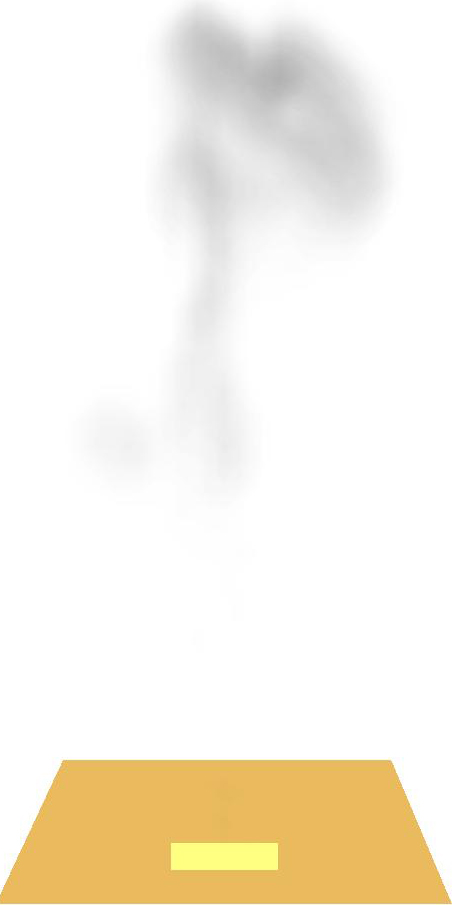
\includegraphics[height=4.0in]{FIGURES/splume_20_27}&
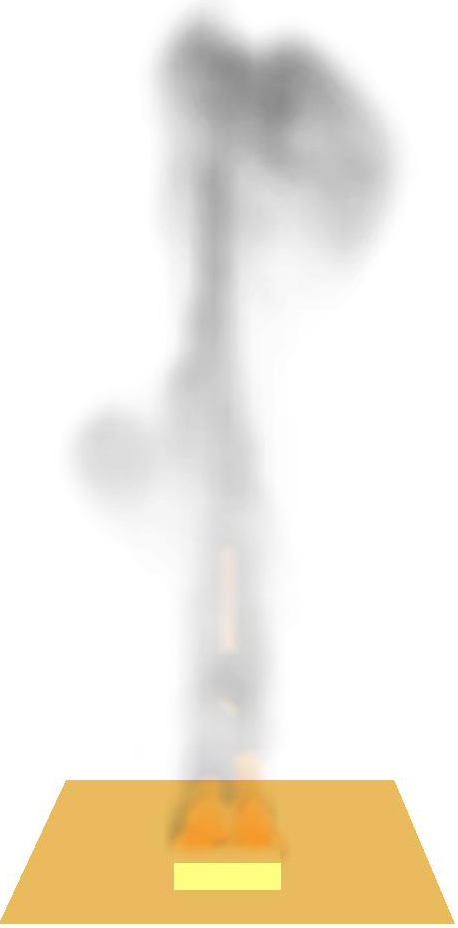
\includegraphics[height=4.0in]{FIGURES/splume_17_27}\\
8 slices&11 slices\\
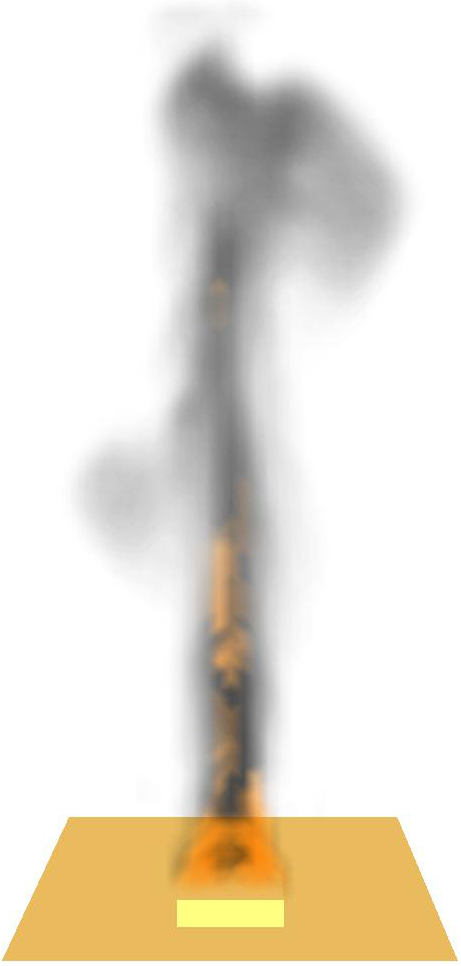
\includegraphics[height=4.0in]{FIGURES/splume_14_27}&
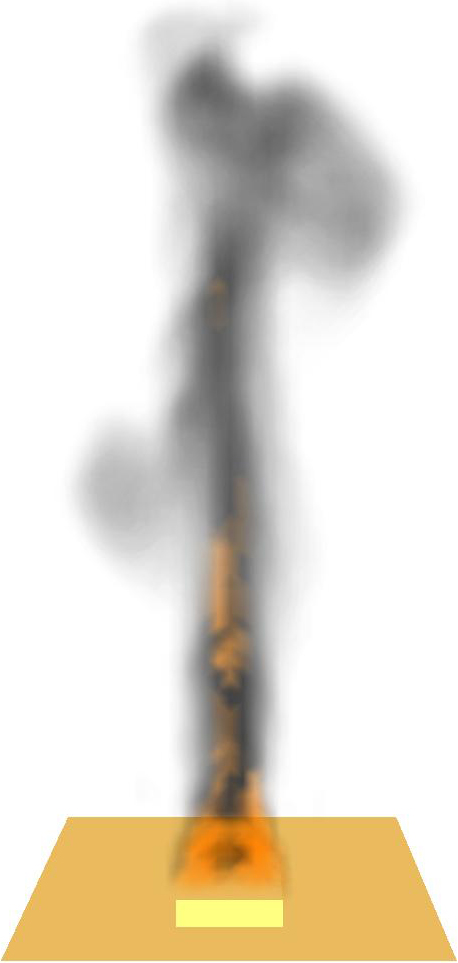
\includegraphics[height=4.0in]{FIGURES/splume_11_27}\\
14 slices&all slices
\end{tabular}
\end{center}
\caption [Smoke plume visualized using several vertical parallel
partially transparent planes.] {Smoke plume visualized using
several vertical parallel partially transparent planes. The smoke
plume looks more realistic as more slice planes are included to
form the image. } \label{figplume}
\end{figure}

\noindent This process is repeated for each smoke plane.

Figure \ref{figsmoke3d} illustrates this process showing smoke and
fire in a townhouse kitchen fire. The visualization is performed
by displaying a series of partially transparent planes. For
illustration, these planes are made more conspicuous (in Fig.
\ref{figsmoke3d}a) by skipping smoke planes (displaying every
third plane) and orienting them along the $x$~axis. Figure
\ref{figsmoke3d}b shows the visualization as it normally appears
with all slice planes shown and oriented along a plane most
perpendicular to the view direction.

\begin{figure}[\figoptions]
\begin{center}
\begin{tabular}{l}
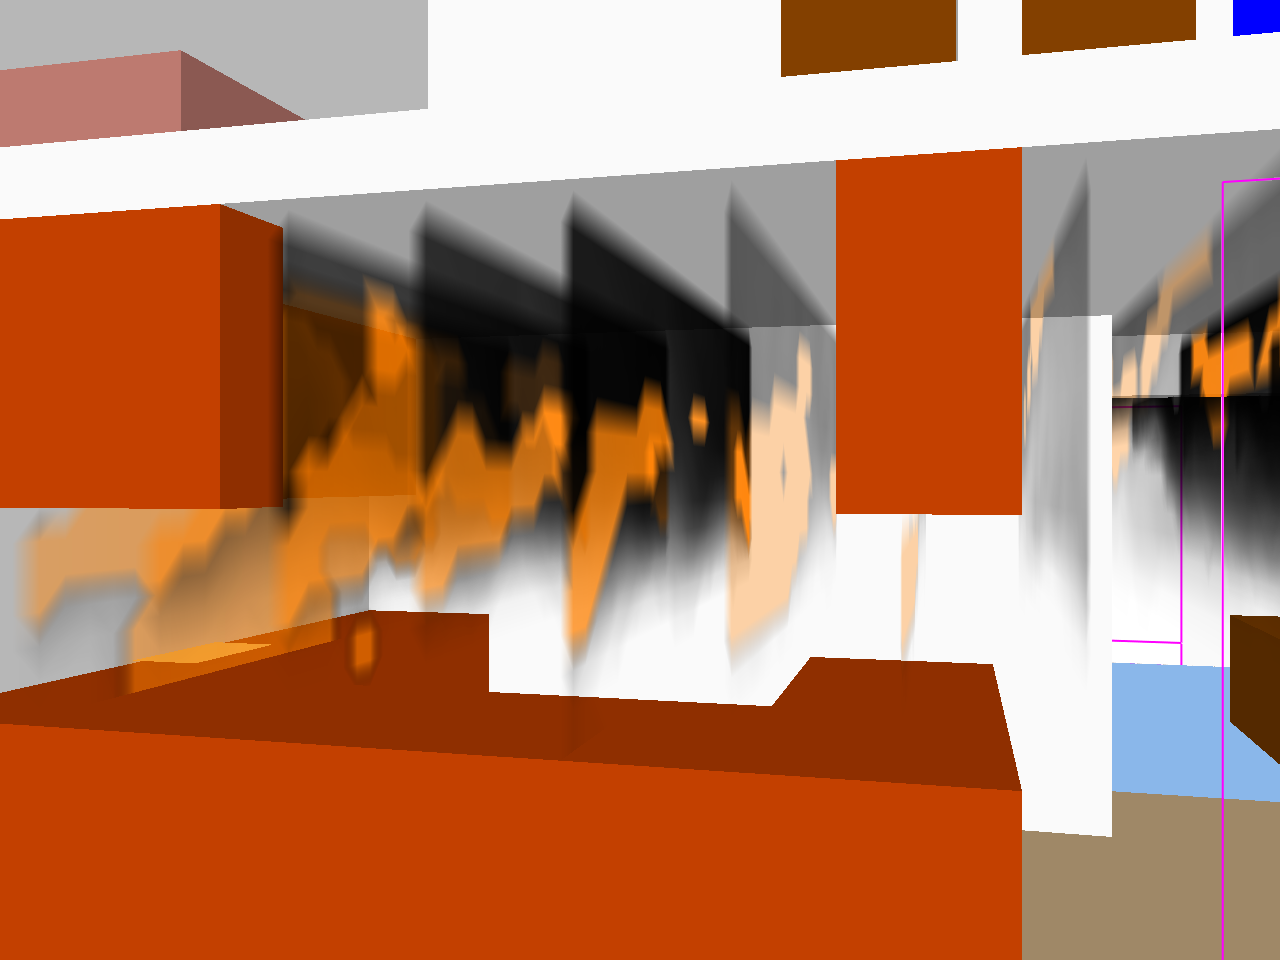
\includegraphics[height=3.75in]{FIGURES/thouse5c_skip}\\
a) slices skipped and oriented along `X' directions\\
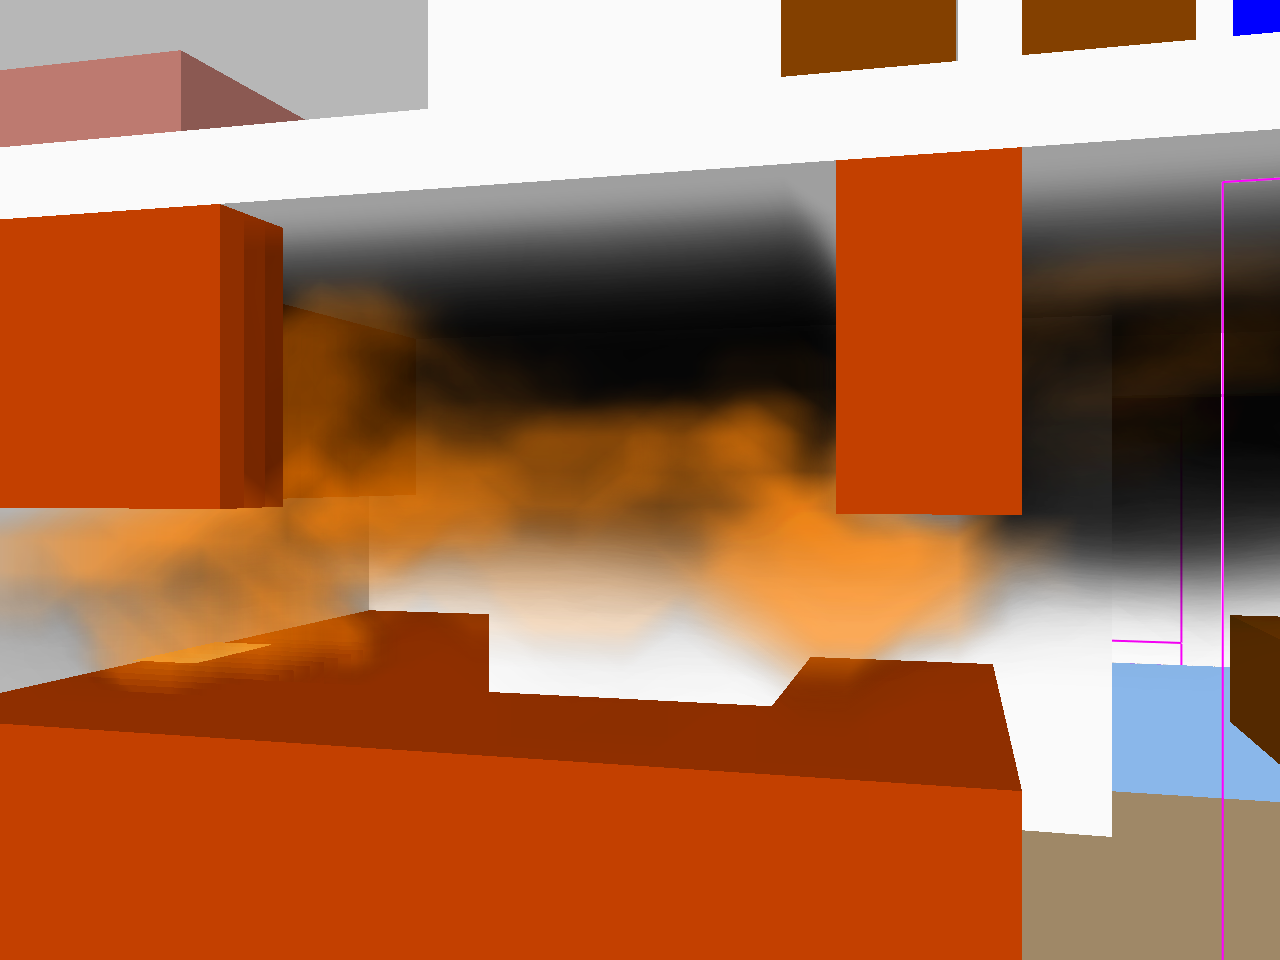
\includegraphics[height=3.75in]{FIGURES/thouse5c_full}\\
b) all slices shown and oriented towards viewer \\
\end{tabular}
\end{center}
\caption[Realistic visualization of a townhouse kitchen fire
simulated using FDS.]{Realistic visualization of a townhouse
kitchen fire simulated using FDS. For illustrative purposes,
planes in the top image are oriented along the $x$~axis.  Planes
in the bottom image are aligned along the $y$~axis, the axis most
perpendicular to the line of sight.}
\label{figsmoke3d}%
\end{figure}

% -------------------  Orienting smoke planes ------------------------

\subsection{Orienting Slice Planes}

Smoke opacity data computed as described in the previous sections
is stored in a 3D array. This array corresponds to the solution
domain as set up in an FDS input file (or some other model). Smoke
planes are drawn in Smokeview through this data.  The orientation
is chosen to be most perpendicular to the viewer's line of sight.
A plane orientation exactly perpendicular to the view direction
could be drawn if one is willing to pay the added CPU cost of
interpolating opacity values between grid nodes.

Figure \ref{figDIRA} illustrates this process showing three view
directions and the corresponding smoke plane orientations that
would be used. Off-axis viewing is minimized by selecting the view
planes orientation that minimizes the angle between the planes
normal direction and the view direction. This angle, $\theta$, is
illustrated in Fig. \ref{figDIRB}, and is given by

\begin{eqnarray}
\cos(\theta)=\frac{n\cdot v_e}{||n||~||v_e||}
\end{eqnarray}

\noindent where $n$ is normal vector for the candidate smoke
plane, and $v_e$ is the view direction vector.  In OpenGL, the
view direction vector, $v_e$, is computed by simply obtaining the
OpenGL modelview matrix, $M$ and multiplying it by the vector,
$(0,0,1)^T$ or equivalently the third row of $M$.

\begin{figure}
\begin{tabular}{ccc}
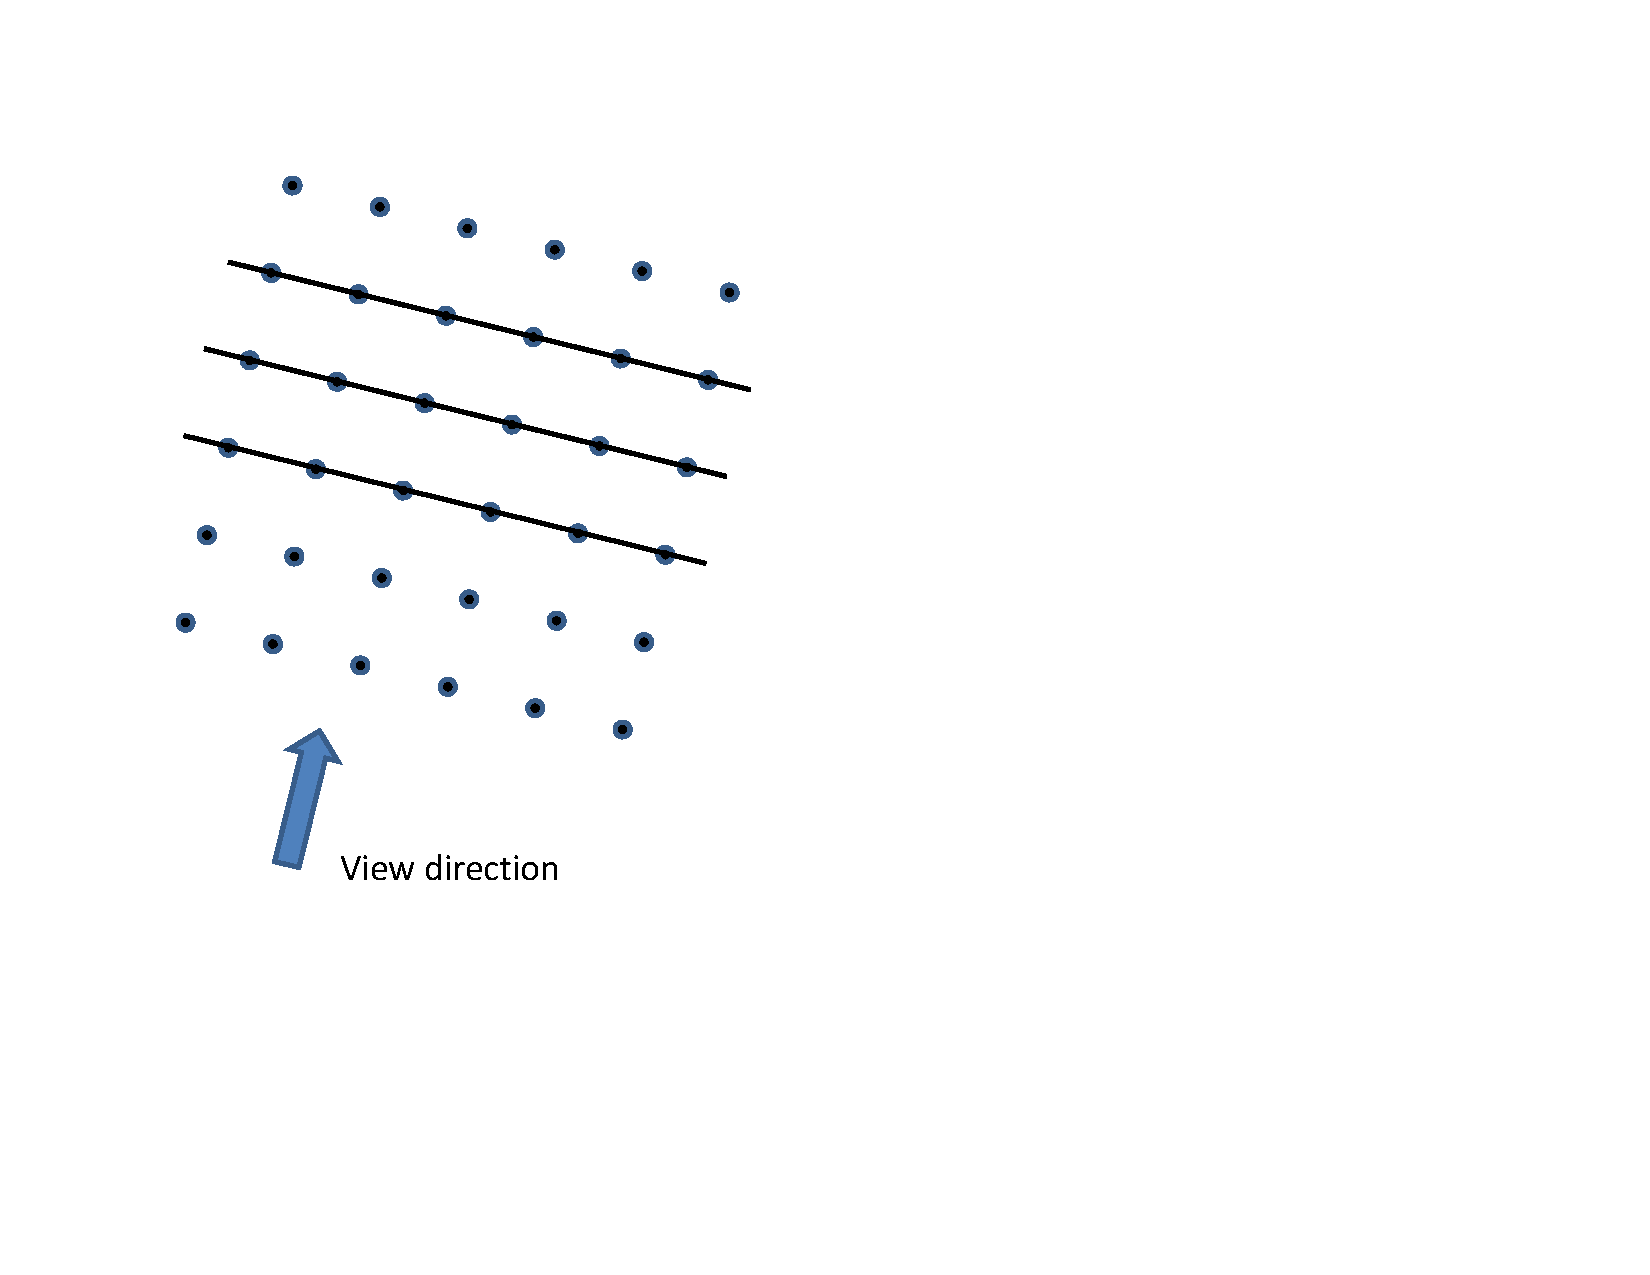
\includegraphics[width=2.25in]{FIGURES/figDIR1a}&
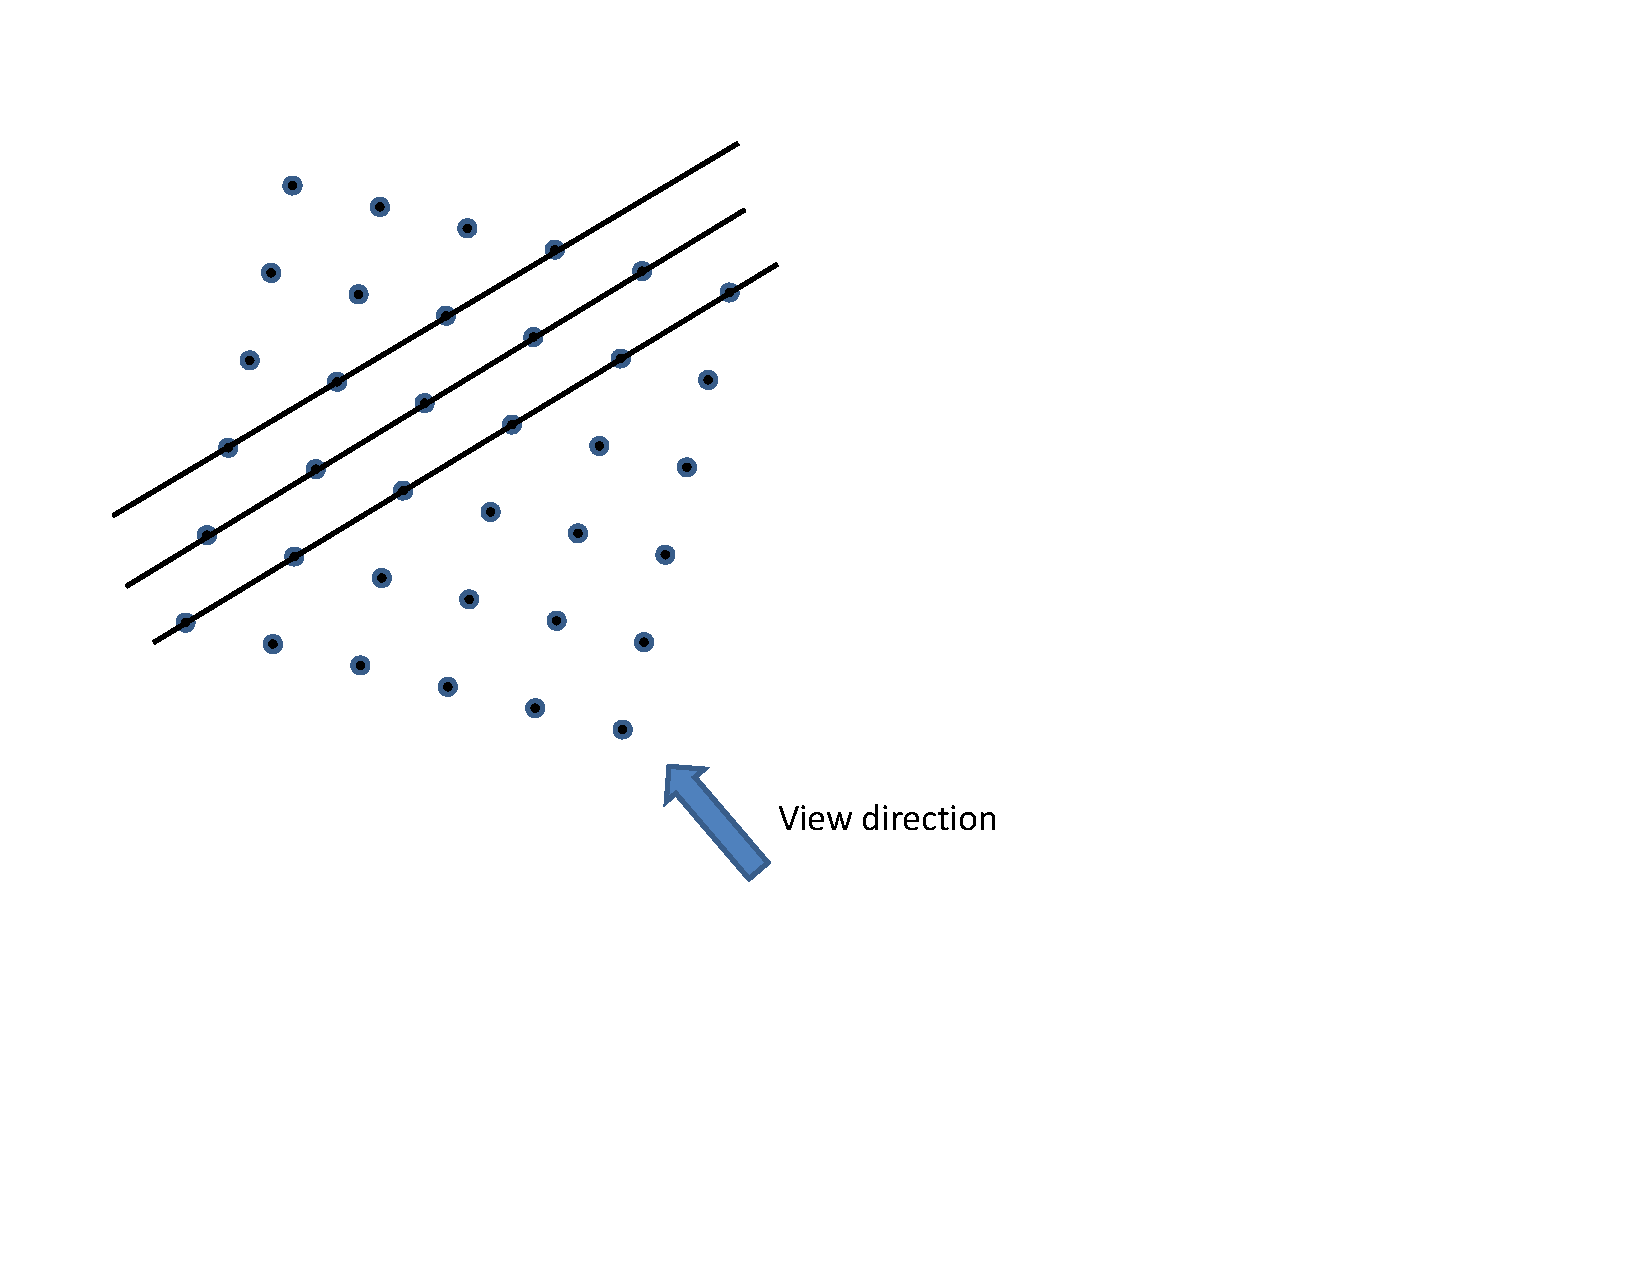
\includegraphics[width=2.25in]{FIGURES/figDIR1b}&
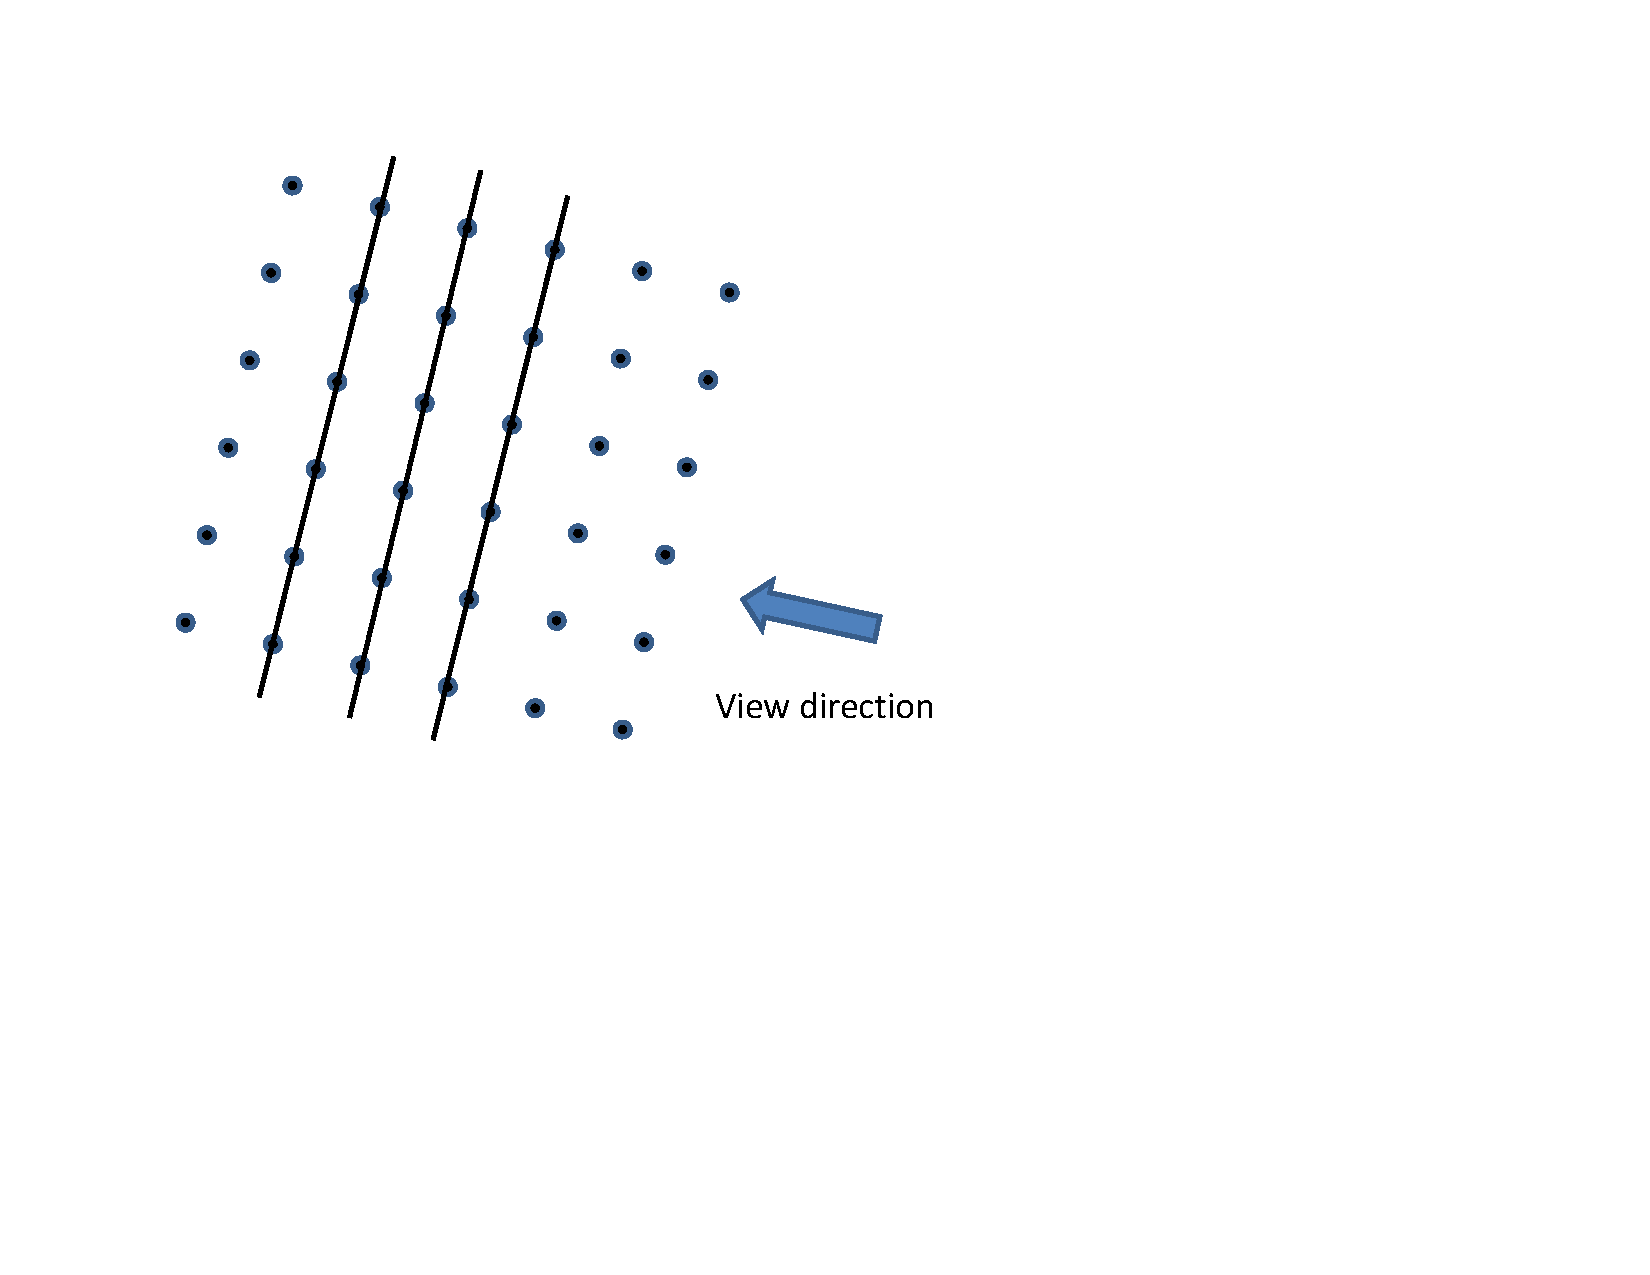
\includegraphics[width=2.25in]{FIGURES/figDIR1c}\\
a) slice planes parallel to the $y$~axis& b) slice planes parallel
to the $y=x$ axis&
c) slice planes parallel to the $x$~axis\\
\end{tabular}
\caption{Slice plane orientation chosen to be {\em most perpendicular}\ to the line of sight }
\label{figDIRA}
\end{figure}

\begin{figure}
\centerline{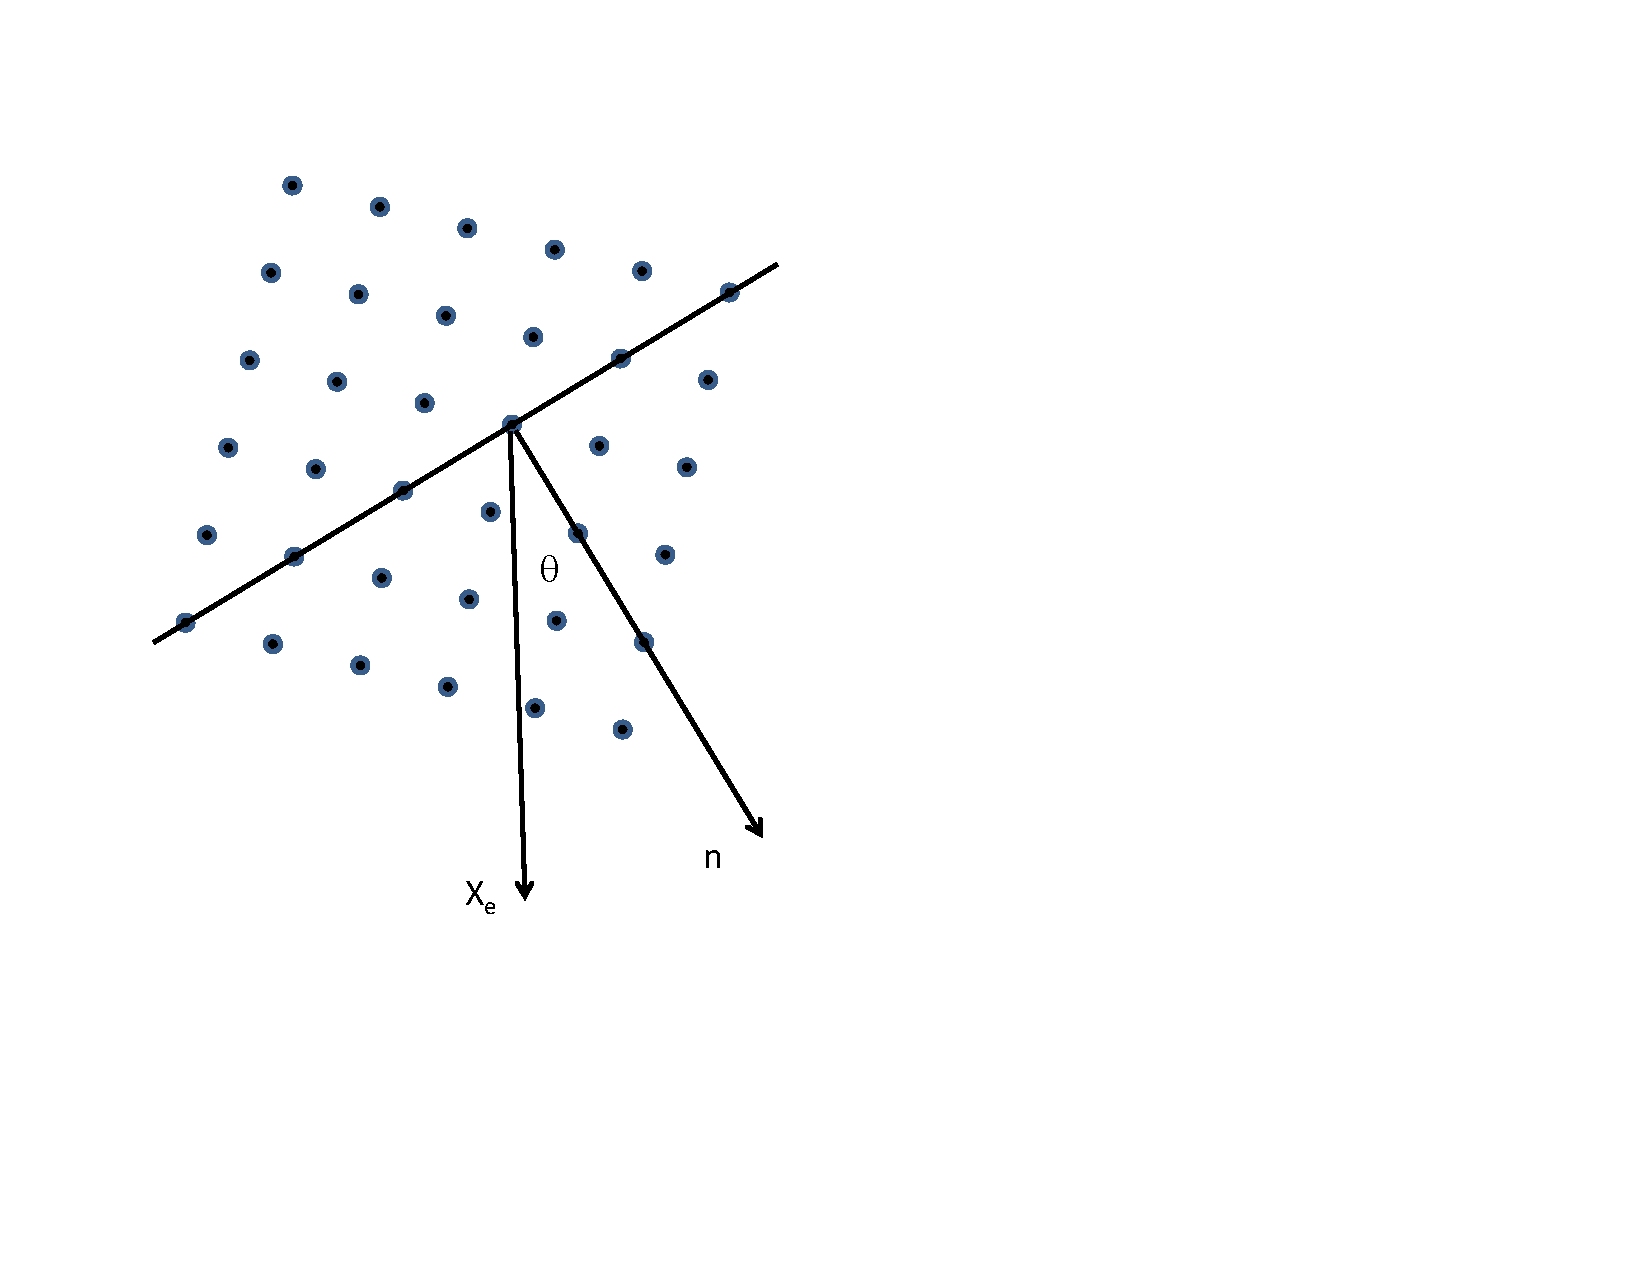
\includegraphics[width=3.0in]{FIGURES/figDIR2}}
\caption[Diagram illustrating the angle between the line of sight
and the vector normal to the slice planes.]{Diagram illustrating
the angle between the line of sight and the vector normal to the
slice planes.  Slice plane orientation is chosen to minimize this
angle.} \label{figDIRB}
\end{figure}

% -------------------  Compressing Slice Plane Data ------------------------

\subsection{Compressing Slice Plane Data}

The opacity parameters are computed at each slice plane node for
all time steps. The space required to store these values can
easily become quite large. Compression techniques are required to
reduce storage requirements.

Storage reduction occurs in two steps.  First, four byte floating
point soot densities are converted to one byte smoke opacities
using the Beer-Lambert law.  Video cards presently use only one
byte to represent opacity. Next, the sequence of opacity values
are compressed using run-length encoding, a compression scheme
where repeated ``runs'' of data are replaced with a number (number
of repeats), and the value repeated.  In more detail,


\begin{enumerate}
\item Represent four or more consecutive identical characters as
$\# n c$ where $\#$ is a special character denoting the beginning
of a repeated sequence, $n$ is the number of repeats and $c$ is
the character repeated.  $n$ can be up to 254 (255 is used to
represent the {\em special}\ character).
\item Represent
characters not repeated four or more times as is.
\end{enumerate}

The character string {\tt aaaaaabbbbcc}\ would then be encoded as
{\tt \#6a\#4bcc}.

Run length encoding provides a reasonably good compression ratio,
is simple to implement and more importantly can be decompressed
quickly. This last property is important for any compression
scheme chosen because it is a rate limiting step in the process
that Smokeview uses to display smoke data. The CPU time required
to compute the smoke flow can easily exceed one minute of CPU time
per output time step, so extra time used to produce a more compact
file is affordable. However, each data frame is decompressed {\em
on the fly}\ so a compression format that can be rapidly
decompressed is critical.

A second compression scheme is used by Smokezip, companion
software to FDS and Smokeview, to more compactly compress FDS
files.  Smokezip uses the ZLIB compression library~\cite{ZLIB}.

% -------------------  A Limitation of the Slice Solution Method ------------------------

\subsection{A Limitation of the Slice Solution Method}
As noted earlier, the slice rendering method for visualizing smoke
records opacities on grid planes using
\begin{equation}
\label{eq:alpha3}
\alpha=1-\exp(-\sigma_t\Delta x)
\end{equation}
where again $\Delta x$ is the distance between adjacent grid
planes.  Problems with round off error can occur because
$\alpha$'s are stored using only 8 bits, the size typical video
hardware uses to represent color and alpha channels. As a result,
opacity values are quantized.  Only values of 0, 1/255, $\cdots$,
254/255 and 1 can be represented.  In particular, any $\alpha$
value computed to be smaller than $1/255$ will truncate to 0. This
can occur when more grid cells are used to resolve a solution
domain, {\em i.e.}\ when $\Delta x$ is sufficiently small so that
$\alpha<1/255$.

For example, suppose that a 1~m column of smoke has opacity of
0.5.  Substituting $\Delta x=1$ and $\alpha=1/2$ into
(\ref{eq:alpha3}) gives $\sigma_t=-\ln(1/2)$.  Solving for $\Delta
x$ using this value of $\sigma_t$ and $\alpha=1/255$ gives
\begin{eqnarray}
\Delta x = \frac{\ln(254/255)}{\ln(1/2)}
\end{eqnarray}
Therefore, the opacity, $\alpha$, will truncate to zero (for this
example) whenever $\Delta x<\ln(254/255)/\ln(1/2)\approx 0.00567$.
Equivalently, the opacity truncates to zero when
$N>\ln(1/2)/\ln(254/255)\approx 177$, where $N$ is the number of
grid planes in the 1~m column of smoke.  Smoke drawn in this
situation will be {\em invisible}.

To overcome this problem, the RTE needs to be solved across the
full 3D data mesh where intermediate smoke opacities are stored
using full precision arithmetic.  One such algorithm is discussed
in the next section.

% -------------------  A Solution using Volumes ------------------------

\section{Volume Rendering}
Volume rendering is the process of visualizing 3D data by
projecting partially transparent colors derived from 3D data onto
a 2D plane forming an image.  An entire volume of data is used to
generate an image rather than just a slice as in the previous
section.  Transfer functions or colormaps are used to map data to
color and optical density (opacity).  In this application
temperature is mapped to color and soot density is mapped to
opacity.  These colors and opacities are then combined to form an
image.  The transfer functions may be arbitrarily designed to
highlight certain portions of the data or based on physics
designed to produce realistic appearing images.  Figure
\ref{figsmokesetup2} illustrates this process. Soot density is
mapped to opacity.  The colors and opacities are then combined to
form an image.  The strategy then is to perform color mixing in
the same way that light would behave by solving an approximate
form of the radiation transport equation.  The approximate RTE
solution given in (\ref{eq:rtesoln})  is used to collapse 3D data
into 2D images projected onto the sides of the mesh visible to the
observer.

\begin{figure}[\figoptions]
\begin{center}
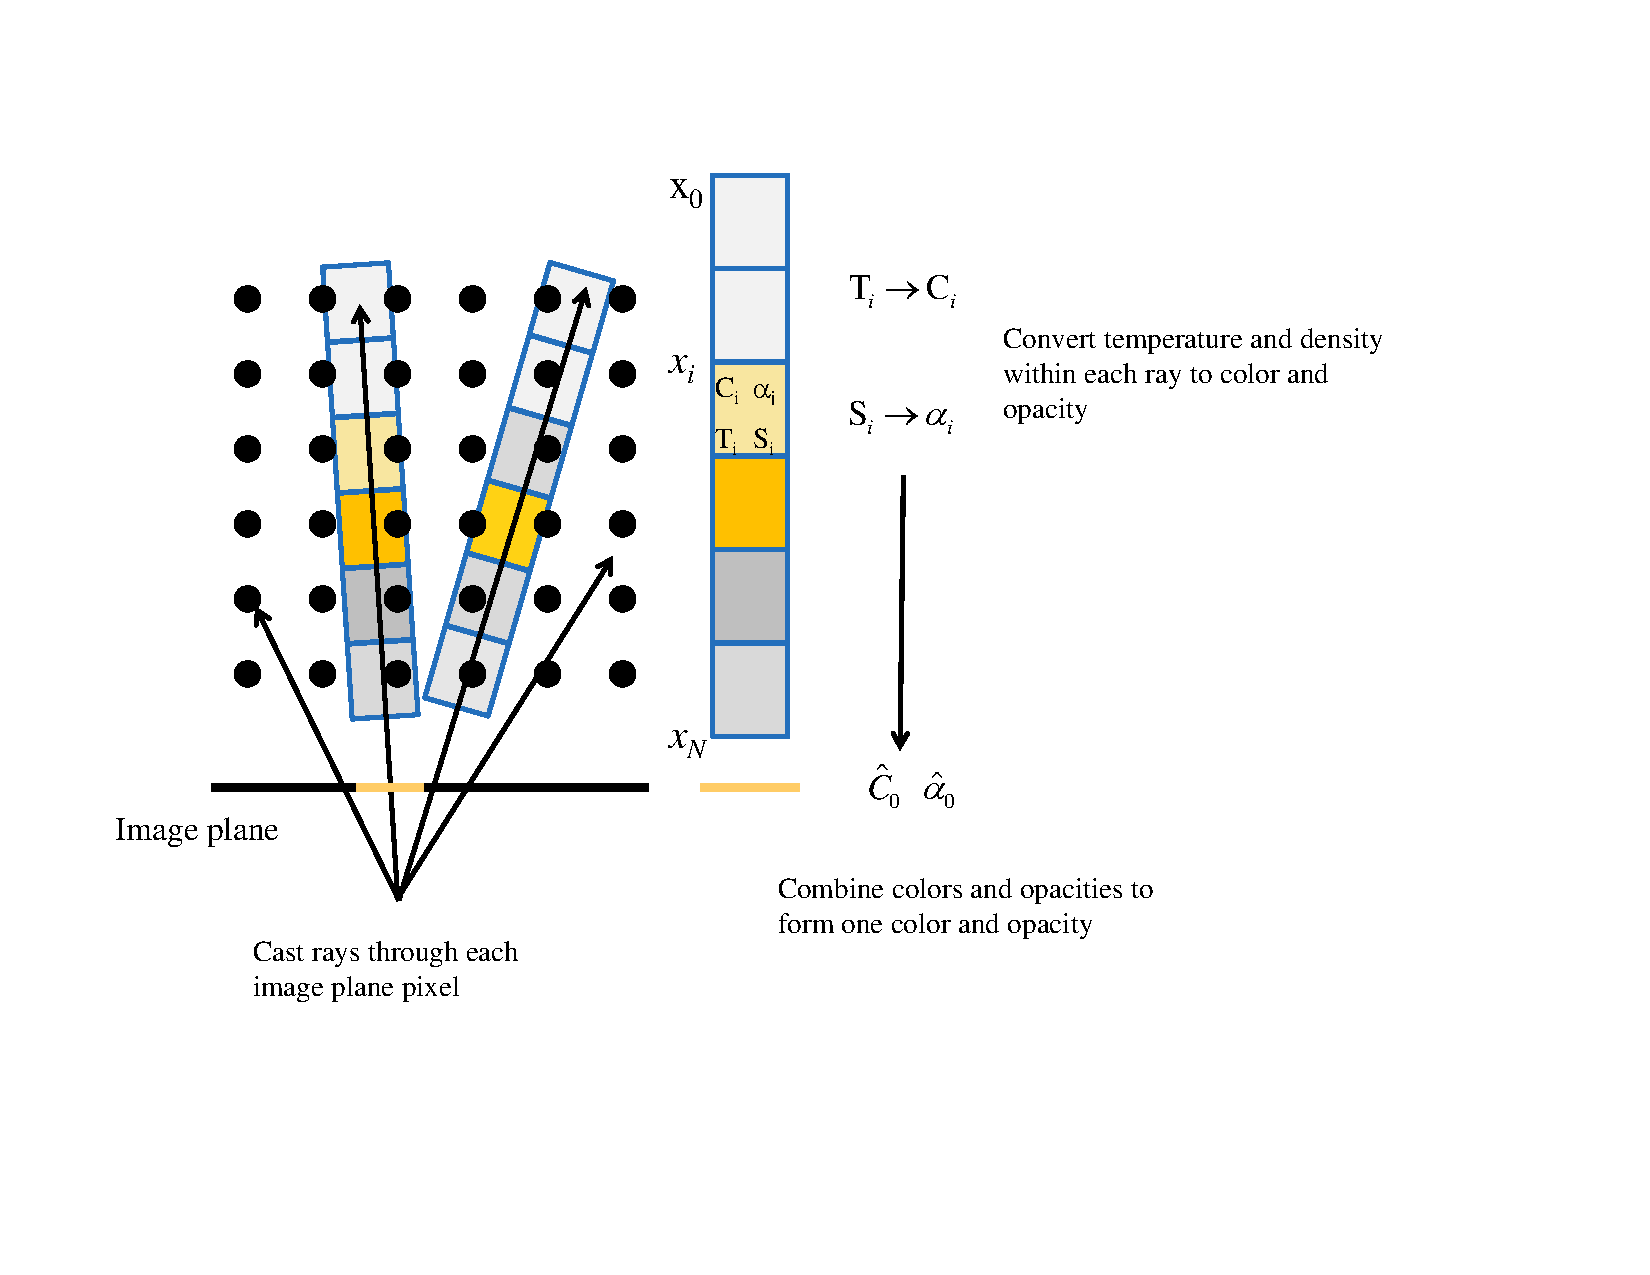
\includegraphics[width=6.5in]{FIGURES/smoke_setup2}
\end{center}
\caption[Opacity and color is computed for each pixel on an image
plane by solving a line integral representation of a simplified
form of the radiation transport equation.]{Opacity and color is
computed for each pixel on an image plane by solving a line
integral representation of a simplified form of the radiation
transport equation.  Rays are cast from the observer through the
image plane into the 3D data set converting temperatures to color
and soot densities to opacity.  The line integral is computed for
each pixel where the ray intersects the data set. }
\label{figsmokesetup2}
\end{figure}

Figure \ref{fig:volplume_example} illustrates the effect of
projecting an image onto a plane.  The top center image is
presented from the point of view of the observer.  The perspective
is correct.  The two images below show the same image but from a
different viewpoint.  The scene is rotated left and right to show
more clearly the images projected on the front facing sides of the
data mesh.  As the scene is moved through rotations and
translations the projected surface images are constantly
recomputed and redrawn presenting the illusion that the image is
3D and drawn within (rather than on the surface) of the data mesh.


\begin{figure}[\figoptions]
\begin{center}
\begin{tabular}{c}
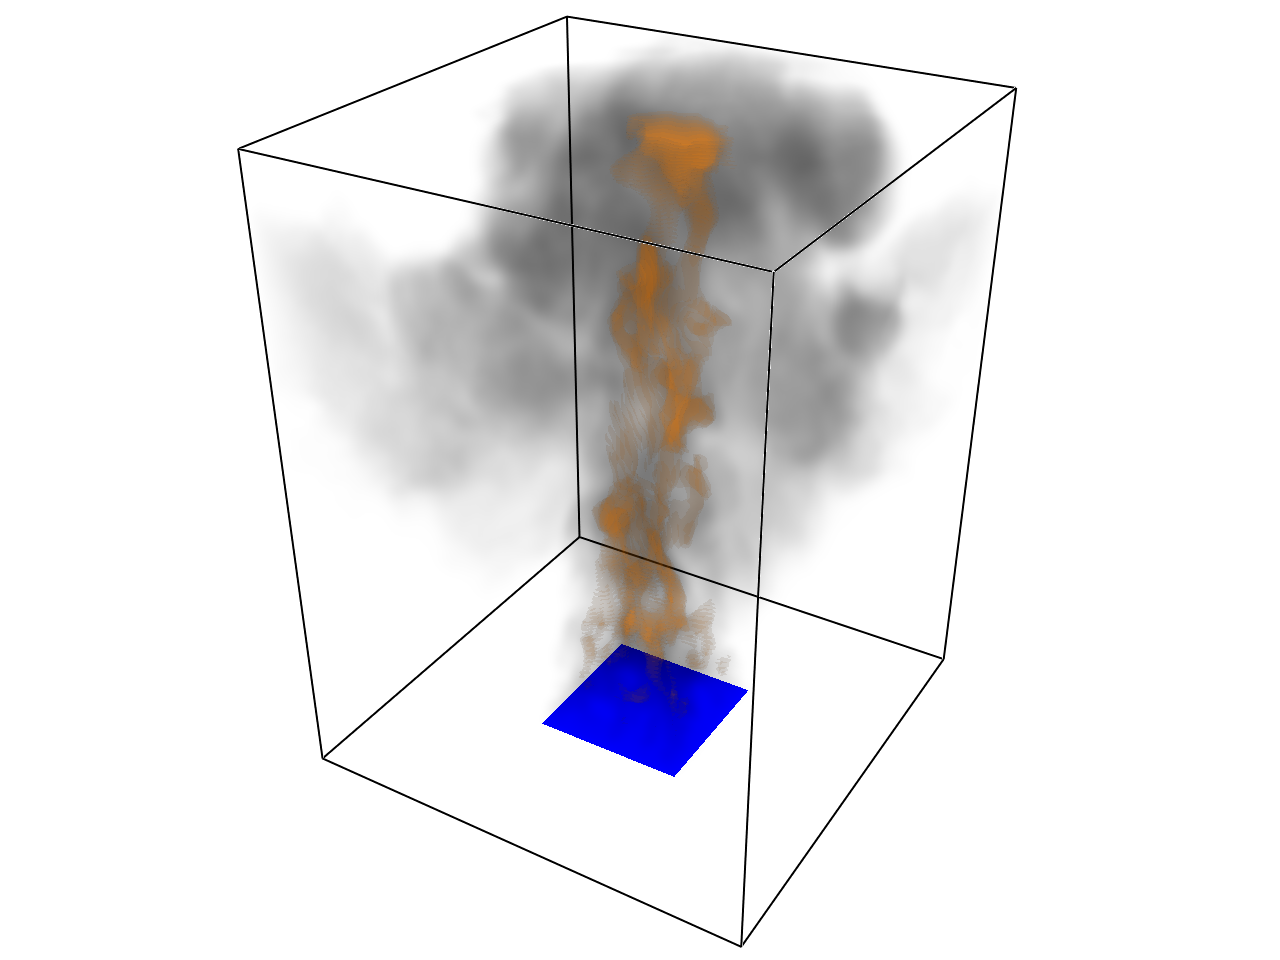
\includegraphics[width=3.5in]{FIGURES/vis_test2_nonfreeze}\\
a) normal view as seen by the observer
\end{tabular}
\begin{tabular}{cc}
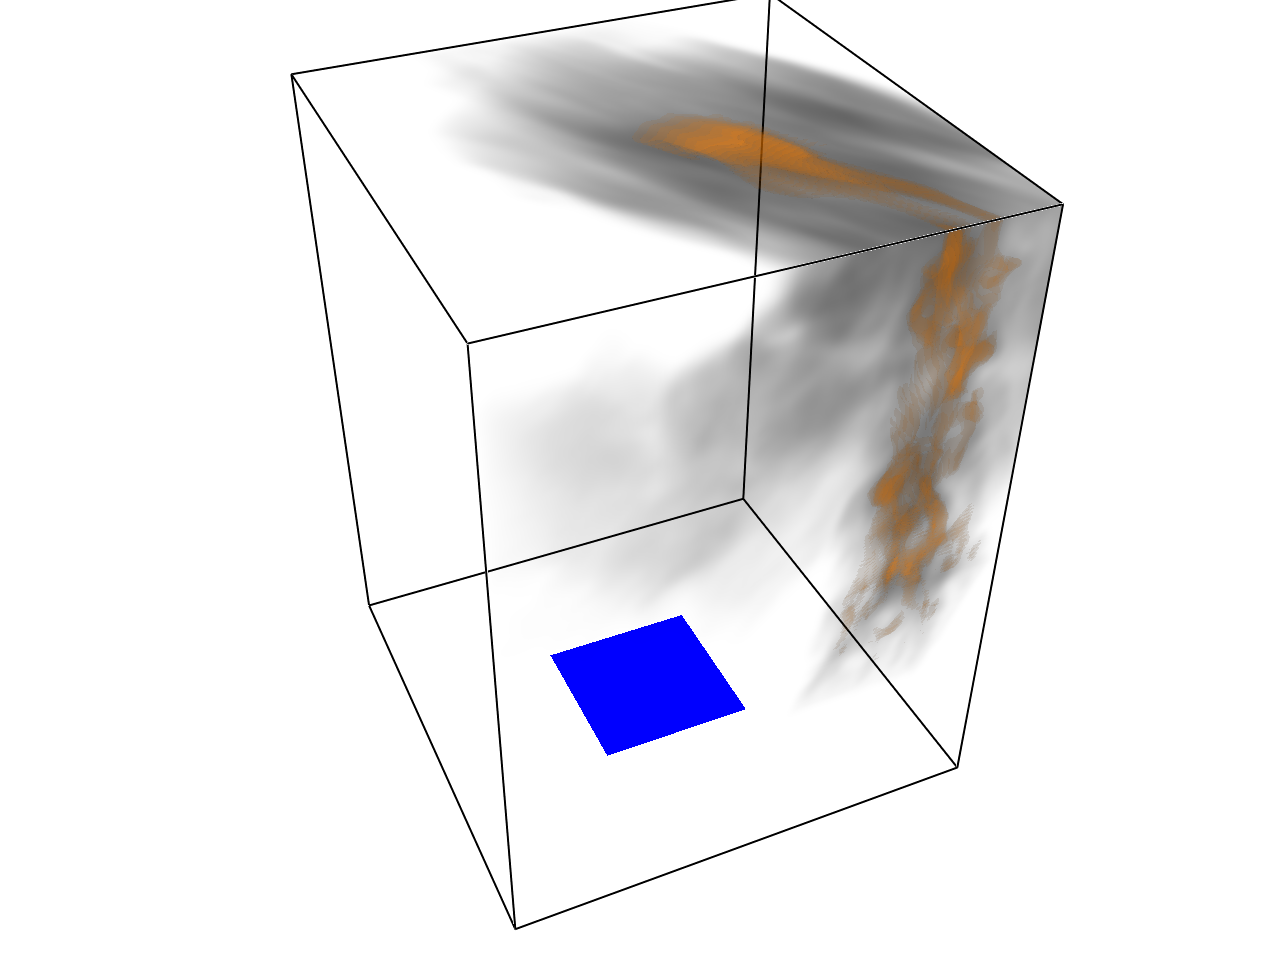
\includegraphics[width=3.5in]{FIGURES/vis_test2_freezeC}&
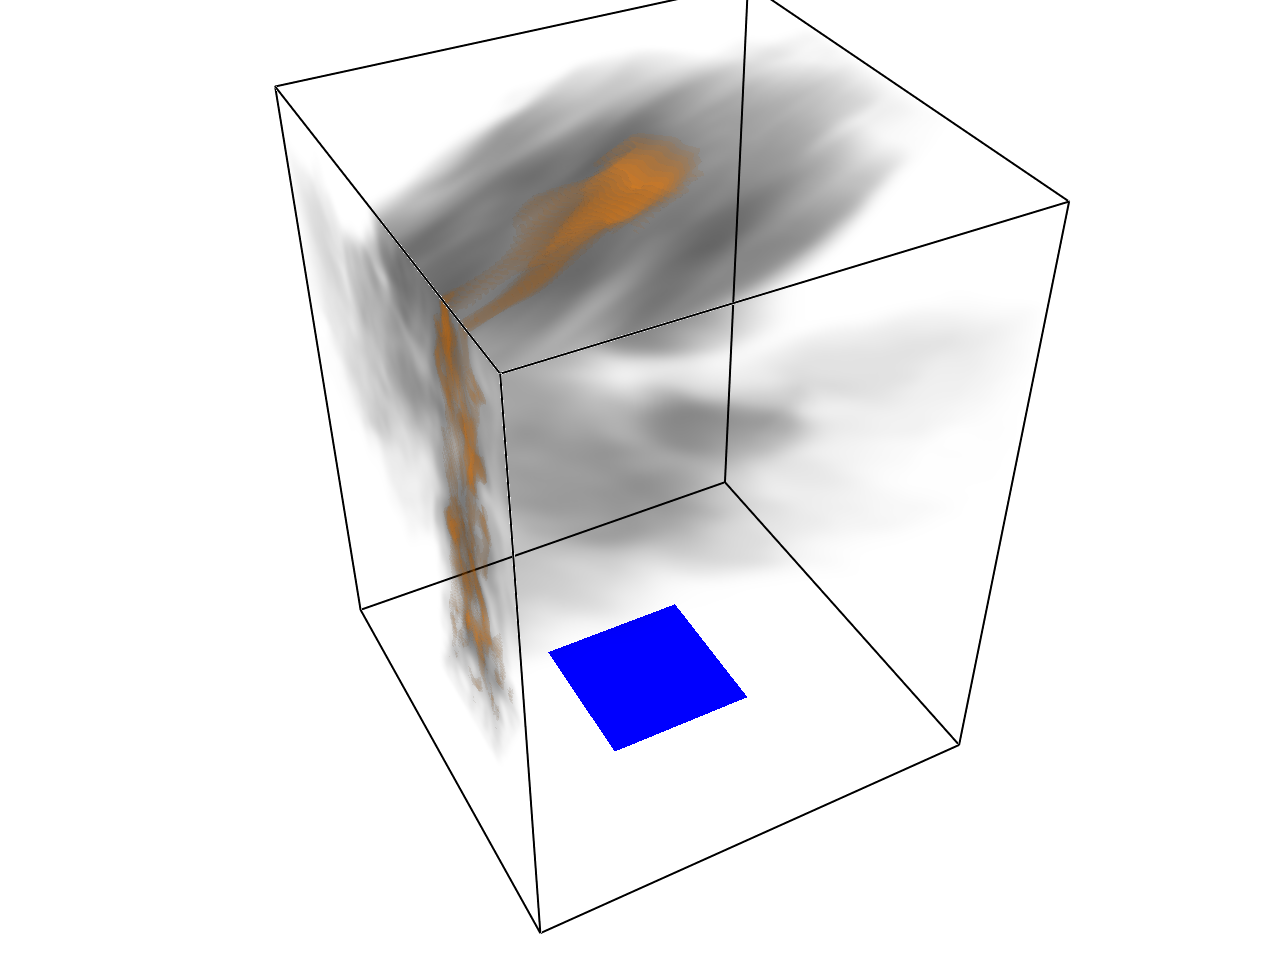
\includegraphics[width=3.5in]{FIGURES/vis_test2_freezeA}\\
b) same image as in a) but viewed from the left&c) same image
as in a) but viewed from the right\\
\end{tabular}
\end{center}
\caption[Volume rendered smoke plume shown from several points of
view.]{Volume rendered smoke plume projected onto the outside
surfaces of the data mesh and shown  from several points of view.
The image, in a), is as viewed by the observer.  The other two
images, b) and c), are rotated versions of the image as in a). }
\label{fig:volplume_example}
\end{figure}

\subsection{Implementation}
Data required to volume render smoke is made available to
Smokeview by adding lines to an FDS input file specifying 3D slice
files for temperature and soot density such as
\begin{lstlisting}
&SLCF XB=xmin,xmax,ymin,ymax,zmin,zmax, QUANTITY='TEMPERATURE' /
&SLCF XB=xmin,xmax,ymin,ymax,zmin,zmax, QUANTITY='DENSITY',SPEC_ID='SOOT' /
\end{lstlisting}
where xmin,~$\cdots$,~zmax represent the domain boundary.

An algorithm for determining image opacities and colors using
volume rendering is detailed below.

\begin{enumerate}

\item For each pixel in the image plane, cast a ray from the
observer's viewpoint through that pixel into the 3D data set

\item Step along the ray from the front (relative to the observer)
to the back of the 3D data set converting data values along the
way to color and opacity.  Choose a step size (possibly varying)
to capture changes occurring in the data set.

\item Combine the colors and opacities found in step 2 using
recursions equations (\ref{eq:alpha2}) and (\ref{eq:color}).
Initiate the recursion with $\hat{\alpha}_{N}=\hat{C}_{N}=0$.
Continue the recursion for $i=N-1$ to $i=0$ by computing
$\hat{\alpha}_i$ and $\hat{C}_i$ using:

\begin{eqnarray}
\hat{\alpha}_i&=&\hat{\alpha}_{i+1}+\left(1-\hat{\alpha}_{i+1}\right)\alpha_i\\
\hat{C}_i&=&\hat{C}_{i+1}+\left(1-\hat{\alpha}_{i+1}\right)C_i
\end{eqnarray}

where $\hat{C}_i$ and $\hat{\alpha}_i$ are color and opacity
accumulated from steps $N$ to $i$ while stepping through the 3D
data set from front to back.  When data is mapped appropriately to
color and opacity, this recursion is simply a numerical
integration of the radiation transport equation. The values $C_i$
and $\alpha_i$ are the color and opacity at the $i$'th step.

\item Mix the volume rendered color, $\hat{C}_N$, with the colors
already rendered using equation (\ref{eq:C_summary}) re-written as

\begin{eqnarray}
\noindent\mbox{updated background color} =
(1-\hat{\alpha}_N)\times \mbox{original background color} +
1\times\hat{C}_N
\end{eqnarray}

The OpenGL call, {\tt
glBlendFunc(GL\_ONE,GL\_ONE\_MINUS\_SRC\_ALPHA); }, is used to
implement this mixing mode in Smokeview.
\end{enumerate}

A limitation of the volume rendering procedure is the large file
sizes required to store the full precision being used in
computations. For example, smoke flow computed on a
128$\times$128$\times$128 mesh for 1024 time steps requires 16
gigabytes to store data for visualization. As with the slice
rendering method, compression procedures are implemented using the
ZLIB library~\cite{ZLIB} to reduce the file size.


% -------------------  Future Work ------------------------

\section{Future Work}
This \paper\ describes the algorithms Smokeview uses to display
smoke and fire using physics based algorithms. These algorithms
may be improved in several ways. Presently, only radiation from
soot is used to visualize smoke. The gray gas assumption may be
relaxed by solving the RTE for several wavelength bands (as may be
done by FDS) and combining the results. The RTE line integration
needs to terminate at the first solid object encountered (FDS
OBST) rather than the far side of the data mesh. The computational
efficiency may be improved by implementing algorithms to skip over
regions with little or no smoke. Research on unstructured
geometries for future incorporation into FDS may also lead to
better visualization. Finally, flame color computations may be
made more quantitative by using a transfer function relating
temperature to color that is physics based rather than an assumed
color map.
